\NeedsTeXFormat{LaTeX2e}[2005/12/01]
%%    2009/03/12 v1.0 GAUBM Vorlage fuer Aschlussarbeiten Physik
%% Template fuer Bachelor- und Masterarbeiten
%% an der Fakultaet fuer Physik (c) Thomas Pruschke der GA Universitaet
%% Verbesserungsvorschlaege bitte an pruschke@theorie.physik.uni-goettingen.de
%%
%% Benoetigte Pakete: datenumber
%%

%%%%%%%%%%%%%%%%%%%%%%%%%%%%%%%%%%%%%%%%%%%%%%%%%%%%%%%%%%%%%%%%%%%%%%
%%%%%%%%%% Bitte vor dem Veraendern diese Datei umbenennen! %%%%%%%%%%
%%%%%%%%%%%%%%%%%%%%%%%%%%%%%%%%%%%%%%%%%%%%%%%%%%%%%%%%%%%%%%%%%%%%%%

%% scrbook - Ersatz fuer LaTeX book Klasse aus dem KOMA Script
%% Moegliche Optionen: diejenigen der Klasse scrbook ausser titlepage

%% deutsche Arbeit:
\documentclass[bachelor,       %% Typ der Arbeit: bachelor oder master
               twoside,        %% zweiseitiges Layout
               BCOR10mm,       %% Bindekorrektur 10 mm
%               liststotoc,nomtotoc,bibtotoc, %% Aufnahme der div. Verzeichnisse
                                              %% ins Inhaltsverzeichnis
               english,ngerman, %% Alternativspr. Englisch, Dokumentspr. Deutsch
%               ngerman,english  %% Alternativspr. Deutsch, Dokumentspr. Englisch
%               final,          %% Endversion; draft fuer schnelles Kompilieren
               ]{GAUBM}

\usepackage{setspace}  %% Zur Setzung des Zeilenabstandes
\usepackage{babel}     %% Sprachen-Unterstuetzung
\usepackage{calc}      %% ermoeglicht Rechnen mit Laengen und Zaehlern
\usepackage[T1]{fontenc}       %% Unterstutzung von Umlauten etc.
%\usepackage[latin1]{inputenc}  %% 
%% in aktuellem Linux & MacOS X wird standardmaessig UTF8 kodiert!
\usepackage[utf8]{inputenc}    %% Wenn latin1 nicht geht ...

\usepackage{amsmath,amssymb} %% zusaetzliche Mathe-Symbole

%für bessere platzierung von bildern etc.
\usepackage{float}

%to use subfigures to create a side-by-side graphic
\usepackage{subcaption}

%added for proofs, theorems etc.
\usepackage{amsthm}
\newtheorem{definition}{Definition}

\usepackage{lmodern} %% type1-taugliche CM-Schrift als Variante zur
                     %% "normalen" EC-Schrift
                     
%% Paket fuer bibtex-Datenbanken
\usepackage[comma,numbers,sort&compress]{natbib}
%for years etc. in the citations use this line:
%\usepackage[sort&compress,square,comma,authoryear, numbers]{natbib}

\bibliographystyle{plainnat}

\newcommand{\tabheadfont}[1]{\textbf{#1}} %% Tabellenkopf in Fett
\usepackage{booktabs}                      %% Befehle fuer besseres Tabellenlayout
\usepackage{longtable}                     %% umbrechbare Tabellen
\usepackage{array}                         %% zusaetzliche Spaltenoptionen

%% umfangreiche Pakete fuer Symbole wie \micro, \ohm, \degree, \celsius etc.
\usepackage{textcomp,gensymb}

\usepackage{mathtools}
\newcommand{\defeq}{\vcentcolon=}
\newcommand{\eqdef}{=\vcentcolon}

%to check for dead references
%\usepackage{refcheck}

%\usepackage{SIunits} %% Korrektes Setzen von Einheiten
%\usepackage{units}   %% Variante fuer Einheiten

%bessere option?
\usepackage{siunitx}

%% Hyperlinks im Dokument; muss als eines der letzten Pakete geladen werden
\usepackage[pdfstartview=FitH,      % Oeffnen mit fit width
            breaklinks=true,        % Umbrueche in Links, nur bei pdflatex default
            bookmarksopen=true,     % aufgeklappte Bookmarks
            bookmarksnumbered=true  % Kapitelnummerierung in bookmarks
            ]{hyperref}

%% Weiter benoetigte Pakete: datenumber
%% Falls dieses Paket nicht in der Installation vorhanden ist,
%% kann es von der Seite mit diesem Template heruntergeladen werden
%% und in einem LaTeX bekanntem Verzeichnis installiert werden (notfalls
%% dem Verzeichnis mit der Arbeit).
\begin{document}
%%
%%                   Ab hier muessen die Anpassungen geschehen
%%
%% Hier den eigenen Namen einsetzen
\ThesisAuthor{Roland Simon}{Zimmermann}
%% Hier den Geburtsort einsetzen
\PlaceOfBirth{Recklinghausen}
%% Titel Arbeit. Das erste Argument ist der deutsche, das zweite der
%% englische Titel.
\ThesisTitle{Spezialisierungspraktikum}{} % second brackets: english title
%% Erst- und Zweitgutacher/in
%% Ist der/die Betreuer/in nicht identisch mit dem/r Erstgutachter/in,
%% muss diese/r als optionales Argument angegeben werden.
\FirstReferee{Prof.\ Dr.\ Ulrich Parlitz}
\Institute{Max-Planck-Institut für Dynamik und Selbstorganisation}
\SecondReferee{nicht vorhanden}
%% Beginn und Ende des Anfertigungszeitraumes
\ThesisBegin{1}{4}{2009}
\ThesisEnd{15}{7}{2009}
%% DO NOT TOUCH THESE LINES!!!!
\frontmatter
\maketitle
\cleardoublepage
%% Zusammenfassung. Falls nicht gewuenscht, bitte auskommentieren.
\begin{abstract}
  Durch die Verwendung von \textit{Echo State Networks} (\textsc{ESNs}) aus dem Bereich des \textit{Reservoir Computings} konnten in der Vergangenheit Fortschritte bei der Vorhersage zeitlicher Signale erreicht werden. In dieser Arbeit werden sie verwendet, um eine raumzeitliche (chaotische) Dynamik in einem zweidimensionalen System vorherzusagen. Dabei soll eine mögliche Verwendung in der Untersuchung von Herzen betrachtet werden. Dazu wird der Ansatz zuerst auf das \textit{Barkley}- und das \textit{Michell-Schaeffer}-Modell, welche beide zur Beschreibung von Herzdynamiken genutzt werden, angewendet, und mit anderen bestehenden Verfahren verglichen. Anschließend wird das komplexere \textit{Bueno-Orovio-Cherry-Fenton}-Modell betrachtet und die vorherigen Erkenntnisse darauf angewendet. Diese Modelle beschreiben ein sogenanntes \textit{erregbares Medium} mit mehreren Systemvariablen.\\
   In der Arbeit werden drei Fragestellungen betrachtet: Als erstes wird eine Kreuzvorhersage zwischen den Systemvariablen durchgeführt. Anschließend wird die Dynamik aus der Kenntnis einer künstlich verschwommenen Messung durchgeführt. Abschließend werden die Erregungen in ungemessenen Arealen aus der Kenntnis der Randwerte dieser durchgeführt. Alle Fragestellungen werden sowohl mit den \textsc{ESN}s, als auch mit den klassischen Methoden der \textit{Nächsten-Nachbar}-Vorhersage und der \textit{radialen Basisfunktionen} als Vergleich, bearbeitet. In allen drei Szenarien erreichen die \textsc{ESN}s eine größere Genauigkeit. Sie können die ersten beiden Aufgaben lösen, aber scheitern an der letzten.  

%% Optional: Stichwoerter. Wenn nicht gewuenscht, koennen die beiden
%% folgenden Zeilen geloescht werden
  \bigskip\par
  \textbf{Stichwörter:} Echo State Network, raumzeitliche Dynamik, Chaos, Herzdynamik, Zeitreihenvorhersage, Kreuzvorhersage
\end{abstract}

\clearpage

%% So laesst sich in die andere Sprache umschalten (Englisch bzw. Deutsch)
\begin{otherlanguage}{english}
\begin{abstract}
  Great progress for the prediction of time series has been made in the past by using \textit{Echo State Networks} (\textsc{ESN}s), which are part of the \textit{reservoir computing}. In this thesis they will be used to predict the spatio-temporal (chaotic) dynamics of a two-dimensional system. Thereby, the possible application for studies of the heart shall be considered. Therefore, at first the \textsc{ESN}s are applied on to the \textit{Barkley} and the \textit{Michell-Schaeffer} model, which both can be used to describe the heart's dynamics, and are compared to existing methods. Later, the \textit{Bueno-Orovio-Cherry-Fenton}-model is investigated and the \textsc{ESN} applied another time using the previously obtained insights. These models describe an \textit{excitable medium} with multiple variables.\\
  Three questions will be studied: In the beginning a cross-prediction between the different variables of the systems will be performed. Next, the real dynamics will be predicted by knowing artificial blurred measurements of those. Finally, the excitations of unmeasured regions of the system will be predicted by measuring the boundary values of those. These questions are analyzed using \textsc{ESN}s; the classical methods of the \textit{next neighbour} prediction and the \textit{radial basis functions} are used to compare the performance. While the \textsc{ESN} approach can solve the first two tasks, it fails the last one. But in all three questions it gains a higher accuracy than the two classical approaches.
  \bigskip\par
  \textbf{Keywords:} Echo State Network, spatiotemporal dynmaics, chaos, dynamics of hearts, prediction of time series, cross prediction
\end{abstract}
\end{otherlanguage}

%% Ende des Vorspanns
\cleardoublepage
%% Ab hier 1 1/2 facher Zeilenabstand (durch setspace-Paket)
\onehalfspacing
%% Erzeugt Inhaltsverzeichnis
\tableofcontents

%% Hier kann man seine Bezeichnungsweisen erklaeren. Falls nicht
%% benoetigt, bis einschliesslich \end{nomenclature} auskommentieren
\begin{nomenclature}
%% Fuer die Berechnung der Spaltenbreiten muss \usepackage{calc}
%% geladen sein!
\section*{Lateinische Buchstaben}
\noindent
\begin{longtable}[l]{p{0.2\textwidth}p{0.7\textwidth-6\tabcolsep}p{0.1\textwidth}}
  \tabheadfont{Variable}&\tabheadfont{Bedeutung}&\tabheadfont{Einheit}\\\midrule\endhead
  $A$ & Querschnittsfl"ache & $\unit{m^2}$\\
  $c$ & Geschwindigkeit & $\unitfrac{m}{s}$
\end{longtable}
\section*{Griechische Buchstaben}
\begin{longtable}[l]{p{0.2\textwidth}p{0.7\textwidth-6\tabcolsep}p{0.1\textwidth}}
  \tabheadfont{Variable}&\tabheadfont{Bedeutung}&\tabheadfont{Einheit}\\\midrule\endhead
  $\alpha$  & Winkel & $\unit{\degree}$; --\\
  $\varrho$ & Dichte & $\unitfrac{kg}{m^3}$
\end{longtable}
\section*{Indizes}
\begin{longtable}[l]{p{0.2\textwidth}p{0.8\textwidth-4\tabcolsep}}
  \tabheadfont{Index}&\tabheadfont{Bedeutung}\\\midrule\endhead
  m & Meridian\\
  $r$ & Radial
\end{longtable}
\section*{Abk"urzungen}
\begin{longtable}[l]{p{0.2\textwidth}p{0.8\textwidth-4\tabcolsep}}
  \tabheadfont{Abk"urzung}&\tabheadfont{Bedeutung}\\\midrule\endhead
  2D & zweidimensional\\
  3D & dreidimensional\\
  max & maximal
\end{longtable}
\end{nomenclature}
%% \listoftables und \listoffigures sollten nur bei genuegender Anzahl Tabellen
%% verwendet werden
%\listoffigures
%\listoftables


\mainmatter   %% Anfang Hauptteil

\section{Einleitung}
Mittels \textit{Neuronaler Netzwerke} konnten in den vergangenen Jahren viele Probleme des \textit{Machine Learnings} und der datenbasierten Ereignisvorhersage gelöst werden. Hierbei hat sich allerdings die Vorhersage von Zeitserien lange Zeit als problematisch erwiesen - dies änderte sich erst, als rekurrente Netzwerke vermehrt genutzt wurden. Eine Form dieser Netzwerke sind die \textsc{Echo State Networks} aus dem Bereich des \textit{Reservoir Computings}. Sie stellen einen vereinfachten Ansatz dar, welche teilweise bemerkenswerte Ergebnisse bei der Analyse und Vorhersage von Zeitserien liefern kann.\\  

Dieser Bericht gibt eine Übersicht über die im Spezialisierungspraktikum gewonnen Erkenntnisse bezüglich \textsc{Echo State Networks}. Hierbei wurden zuerst die theoretischen Grundlagen betrachtet und die hierbei gewonnenen Informationen anschließend auf zwei Anwendungsbeispiele bezogen.\\

Alle Programmierbeispiele während des Praktikums wurden in \textsc{Python} mittels \textsc{numpy} und \textsc{scipy} erstellt. Die relevanten Auszüge hiervon sind im Anhang zu finden.
\chapter{Theorie}
\label{ch:theory}
Zu Beginn der Arbeit werden zunächst die zwei Modelle zur Beschreibung der Herzdynamik eingeführt, auf die die verschiedenen Ansätze angewendet werden. Im Anschluss daran werden zunächst die theoretischen Grundlagen der klassischen Methoden der \textit{nächsten Nachbar} Vorhersage und der \textit{radialen Basisfunktionen} zusammengefasst. Darauffolgenden wird der Ansatz des \textit{Reservoir Computings} eingeführt und theoretisch anhand der \textit{Echo State Networks} beschrieben.

\section{Modelle des Herzens}
Zur Beschreibung der Herzdynamik existieren verschiedene Modelle. In dieser Arbeit werden zuerst das \textit{Barkley}- und das \textit{Mitchell-Schaeffer}-Modell verwendet, um die Leistungsfähigkeit der \textsc{ESN}s zu überprüfen und einzuordnen. Anschließend werden die gewonnenen Erkenntnisse auf das kompliziertere \textit{Bueno-Orovio-Cherry-Fenton}-Modell angewendet. Im Folgenden sollen die drei Modelle vorgestellt werden.

\subsection{Barkley-Modell}
Das \textit{Barkley}-Modell, welches 1990 von Dwight Barkley vorgestellt wurde, ist ein System aus gekoppelten Reaktionsdiffusionsgleichungen. Dies sind partielle Differentialgleichungen (\textit{PDE}) zweiter Ordnung, welche einen Diffusionsterm besitzen. Das \textit{Barkley}-Modell beschreibt ein erregbares und oszillierendes Medium. Das Modell besteht aus zwei Variablen $u(t)$, $v(t)$ die den  \textit{PDEs}
\begin{equation}
\begin{gathered}
\frac{\partial u}{\partial t} = D \cdot \nabla^2 u + \frac{1}{\epsilon} (1-u) \left(u-\frac{v+b}{a}\right)\\
\frac{\partial v}{\partial t} = u^\alpha-v,
\end{gathered}
\end{equation}
unterliegen \citep{Barkley:2008}. Dabei ermöglicht $\alpha=1$ dem System \textit{periodische} Wellenmuster auszubilden und $\alpha=3$ bedingt ein \textit{chaotisches} Verhalten. Im Folgenden wird stets der Fall $\alpha=3$ betrachtet. Die Variable $u(t)$ durchläuft hierbei eine schnellere Dynamik als die hemmende Variable $v(t)$ \citep{Barkley:2008, berg2011synchronization}. Das Modell kann genutzt werden, um die Dynamik der Herzgewebes zu beschreiben. Dabei nimmt die Variable $u$ die Rolle einer Membranspannung ein.\\
Die Parameter $\epsilon, b$ und $a$ charakterisieren das Verhalten des Systems und werden in der gesamten folgenden Arbeit nach \citep{Barkley:2008} als
\begin{align*}
a &= 0.8,\\ b &= 0.01,\\ \epsilon &= 0.02
\end{align*}
festgelegt.\\
Zudem wird das Modell in dieser Arbeit in zwei Dimensionen betrachtet, sodass $u(t, x,y)$ und $v(t, x,y)$ skalare zeitabhängige Felder sind.\\
Die \textit{PDE}s werden zunächst zur Simulation des Systems zeitlich mit einem Zeitschritt $\Delta t$ und örtlich mit einer Gitterkonstante $\Delta x$ diskretisiert. Zur Beschreibung des Diffusionstermes wird eine Fünf-Punkte Methode
\begin{align}
\nabla^2 u(t)_{i,j} \simeq \frac{u(t)_{i-1, j} + u(t)_{i+1,j} + u(t)_{i,j-1} + u(t)_{i,j+1} - 4 u(t)_{i,j}}{\Delta x^2} \eqdef \Sigma(t)_{i,j}
\end{align} 
nach \citep{Barkley:2008} verwendet. Die tiefergestellten Indizes stehen für den diskretisierten Ort der \textit{x-y-Ebene}.
Für kleine Zeitschritte $\Delta t$ ist ein \textit{explizites Eulerverfahren}
\begin{equation}
\begin{gathered}
u(t+1)_{i,j} = u(t)_{i,j} + \Delta t \cdot \frac{\partial u}{\partial t},\\
v(t+1)_{i,j} = v(t)_{i,j} + \Delta t \cdot \frac{\partial v}{\partial t}
\end{gathered}
\end{equation}
mit

\begin{equation}
\begin{gathered}
\frac{\partial u}{\partial t}_{i,j} = D \cdot \Sigma(t)_{i,j} + \frac{1}{\epsilon} (1-u(t)_{i,j}) \left(u(t)_{i,j}-\frac{v(t)_{i,j}+b}{a}\right)\\
\frac{\partial v}{\partial t}_{i,j} = u(t)_{i,j}^3-v(t)_{i,j}
\end{gathered}
\end{equation}
ausreichend genau. Hierbei werden \textit{Neumann}-Randbedingungen genutzt, sodass die senkrechte Komponente der räumlichen Ableitung an den Rändern des Feldes verschwindet. Im Folgenden wird zudem, in Analogie zu \citep{berg2011synchronization}, die Diffusionskonstante auf $D = 1/25$, die Gitterkonstante auf $\Delta x = 0.1$ und die Zeitkonstante auf $\Delta t = 0.01$ gesetzt. Die raumzeitliche Dynamik des Systems ist in Form der $u$-Variable im Anhang in Abbildung \ref{fig:apx_barkley_evolution} dargestellt.
\section{Mitchell-Schaeffer Modell}
Das \textit{Mitchell-Schaeffer Modell} ist ebenso wie das \textit{Barkley Modell} ein System aus gekoppelten partiellen Differentialgleichungen. Es ist vorgeschlagen worden, um eine phänomenologisches Beschreibung der Aktionspotentiale auf der Membran von Herzzellen zu liefern. Das Modell wird durch die Membranspannung $v(t)$ und eine Kontrollvariable $h(t)$, welche das Verhalten der beteiligten Ionenkanäle steuert, definiert. Hierbei wird die Spannung als dimensionslose Größe dargestellt, die Werte zwischen $0$ und $1$ annehmen kann \citep{mitchell2003two}.\\

Diese Dynamik wird durch die Gleichungen 
\begin{equation}
\begin{gathered}
\frac{\partial v}{\partial t} = \nabla \cdot (D \nabla v) + \frac{h v^2(1-v)}{\tau_{in}} - \frac{v}{\tau_{out}},\\
\frac{\partial h}{\partial t} =
\begin{cases}
	\frac{1-h}{\tau_{open}},& \text{wenn } v \leq v_{gate}\\
    \frac{-h}{\tau_{close}},& \text{wenn } v \geq v_{gate}
\end{cases}
\end{gathered}
\end{equation}
beschrieben. Dabei stehen die Parameter $\tau_{in}, \tau_{out}, \tau_{open}, \tau_{close}$ für Zeitkonstanten, welche die Form des Aktionspotentials modifizieren. Die ersten beiden Konstanten beschreiben die Geschwindigkeit, mit der die Ionen durch die Membran strömen, und die letzten beiden die Geschwindigkeit mit der sich die verantwortlichen Ionenkanäle öffnen beziehungsweise schließen. Zusätzlich stellt die Konstante $v_{gate}$ eine Grenzspannung dar. Beim Über- und Unterschreiten dieser Grenze ändert sich der der jeweilige Zustand der Ionenkanäle , indem $h(t)$ angepasst wird. Im Rahmen dieser Arbeit werden, soweit keine anderen Angaben vorhanden sind, die Parameter durch die Werte aus Tabelle \ref{tab:ms_parameters} in Analogie zu \citep{mitchell2003two} festgesetzt. Dabei ist allerdings $\tau_{open}$ auf $20$ \citep[S. 134ff.]{bartocci2016computational} reduziert worden, da mit dieser Wahl ein chaotischeres Verhalten, ähnlich zum \textit{Barkley-Modell}, erzeugt wird. Dies erschwert die mögliche Vorhersage der Entwicklung, wodurch eine anspruchsvolle Herausforderung erzeugt wird.\\

\begin{table}[H]
\centering
\begin{tabular}{|c|c|c|c|c|}
$\tau_{in}$ & $\tau_{out}$ & $\tau_{open}$ & $\tau_{close}$ & $v_{gate}$ \\ 
\hline 
\hline 
0.3 & 6.0 & 20 & 150 & 0.13 \\ 
\hline 
\end{tabular} 
\caption{Verwendete Zeitkonstaten und Grenzspannung $v_{gate}$ für die Betrachtung des \textit{Mitchell-Schaeffer Modells}}
\label{tab:ms_parameters}
\end{table}

Der erste Summand der zeitlichen Ableitung von $v$ beschreibt ein Diffusionsverhalten, welches durch die Diffusionsmatrix $\mathbf{D} = \text{diag}(D_x, D_y)$ beschrieben wird. Die Einführung dieser Matrix erlaubt im Allgemeinen die Verwendung von zwei verschiedenen Diffusionskontanten $D_x, D_y$, welche Richtungsabhängig sind \citep{talbot2013towards}. Im Folgenden wird für diese allerdings der gleichen Wert $D_x = D_y = D$ gesetzt.\\

Die meisten, auf zellulärer Ebene aufgestellten, Gleichungen haben eine hohe Komplexität. Hierdurch werden numerische Berechnungen sehr aufwendig. In der Herleitung dieses Modells sind einige vereinfachende Annahmen eingeflossen, wodurch die Komplexität und somit auch der numerische Aufwand reduziert worden sind. Trotz des phänomenologischen Charakters des \textit{Mitchell-Schaeffer Modells} besitzen die Parameter eine physiologische Interpretation. Zudem ist es in der Lage wichtige Eigenschaften des Aktionspotentials im Vergleich zu anderen Modellen gut wiederzugeben \citep{talbot2013towards}.\\

Analog zu der Betrachtung des \textit{Barkley Modells} sind für die numerische Betrachtung die beiden \textit{PDE}s erneut in einem expliziten Verfahren mittels
\begin{equation}
\begin{gathered}
\frac{\partial v}{\partial t}_{i,j} = D \cdot \Sigma(t)_{i,j} + \frac{h(t)_{i,j} v(t)_{i,j}^2(1-v(t)_{i,j})}{\tau_{in}} - \frac{v(t)_{i,j}}{\tau_{out}}\\
\frac{\partial h}{\partial t}_{i,j} = \begin{cases}
	\frac{1-h(t)_{i,j}}{\tau_{open}},& \text{wenn } v(t)_{i,j} \leq v_{gate}\\
    \frac{-h(t)_{i,j}}{\tau_{close}},& \text{wenn } v(t)_{i,j} \geq v_{gate}
\end{cases}
\end{gathered}
\end{equation}
diskretisiert worden. Dabei werden im Folgenden die Integrationskonstanten $\Delta x = 0.1, \Delta t = 0.01$ und die Diffusionskonstante $D_x = D_y = D = \num{5e-3}$ genutzt.\\
\subsection{Bueno-Orovio-Cherry-Fenton-Modell}
Ebenso wie die beiden vorherigen Modelle ist das \textit{Bueno-Orovio-Cherry-Fenton}-Modell (\textit{BOCF}-Modell) ein System aus gekoppelten partiellen Differentialgleichungen. Es ist ein sogenanntes \textit{minimales Modell} zur Beschreibung der Aktionspotentiale auf der Membran von Herzzellen. Dies bedeutet, dass nicht jeder einzelne Ionenstrom modelliert wird, sondern diese in drei verschiedene Gruppen unterteilt und diese dann zusammen modelliert werden: Dabei werden sie in \textit{schnell hineinströmende}, \textit{langsam hineinströmende} und \textit{ausströmende} Ionen unterteilt. Dieses Vorgehen reduziert die Anzahl der benötigten Variablen des Systems sehr stark: Während andere Modelle auf Ionenebene zur Beschreibung der Aktionspotentiale viele Variablen besitzen, wie beispielsweise das \textit{Tuscher-Noble-Noble-Panfilov}-Modell (\textit{TNNP}-Modell) mit $17$ Variablen, benötigt das \textit{BOCF}-Modell nur $4$ Variablen - dies senkt den benötigten Rechenaufwand. Gleichzeitig beinhaltet es $28$ Konstanten, welche die Form der Dynamik charakterisieren. Dadurch ist zum einen eine Anpassung an verschiedene experimentelle Messergebnisse möglich, zum anderen können auch die Ergebnisse anderer bestehender Modelle reproduziert werden. Hierdurch kommt die Bezeichung des \textit{minimalen Modells} zustande \citep{Bueno-Orovio2008}.\\

Die Dynamik wird durch die Gleichungen 
\begin{align}
\begin{aligned}
\frac{\partial u}{\partial t} &= D \nabla^2 u - (J_{si} + J_{fi} + J_{so})\\
\frac{\partial v}{\partial t} &= \left(1-H(u-\theta_w)\right)(v_\infty - v)/\tau_v^- - H(u-\theta_v)v/\tau_v^+ \\
\frac{\partial w}{\partial t} &= (1-H(u-\theta_w))(v_\infty - w)/\tau_v^- - H(u-\theta_w)v/\tau_w^+ \\
\frac{\partial s}{\partial t} &= ((1 + \tanh(k_s(u-u_s)))/2 - s)/\tau_s
\end{aligned}
\end{align}
beschrieben. Die drei Ströme $J_{si}$, $J_{fi}$ und $J_{so}$ folgen den Gleichungen
\begin{align}
\begin{aligned}
J_{si} &= -H(u-\theta_w)ws/\tau_{si} \\
J_{fi} &= -vH(u-\theta_v)(u-\theta_v)(u_u - u)/\tau_{fi} \\
J_{so} &= (u-u_o)(1-H(u-\theta_w))/\tau_o + H(u-\theta_w)/\tau_{so}.
\end{aligned}
\end{align}

Dabei steht $H(x)$ für die \textit{Heaviside-Funktion}. Zusätzlich werden sieben spannungsabhängige Konstanten
\begin{align}
\begin{aligned}
\tau_v^-   &= (1-H(u-\theta_v^-))\tau_{v1}^- + H(u-\theta_v^-)\tau_{v2}^- \\
\tau_w^-   &= tau_{w1}^- + (\tau_{w2}^- - \tau_{w1}^-)(1+\tanh(k_w^-(u-t_w^-)))/2 \\
\tau_{so}^- &= tau_{so1}^- + (\tau_{so2}^- - \tau_{so1}^-)(1+\tanh(k_{so}^-(u-t_{so})))/2 \\
\tau_s^-    &= (1-H(u-\theta_w))\tau_{s1} + H(u-\theta_w)\tau_{s2} \\ 
\tau_o^-    &= (1-H(u-\theta_o))\tau_{o1} + H(u-\theta_o)\tau_{o2} \\\\
v_\infty &= \begin{cases}
	1,& \text{wenn } u \leq \theta_v^-\\
    0,& \text{wenn } u \geq \theta_v^-
\end{cases} \\
w_\infty &= (1-H(u-\theta_o))(1-u/\tau_{w\infty}) + H(u-\theta_o)w_\infty^*
\end{aligned}
\end{align}
eingeführt. In diesem Modell beschreibt die Variable $u(t)$ die Membranspannung. Des Weiteren wird das Modell durch $28$ Konstanten charakterisiert. In dieser Arbeit wird der Satz von Konstanten genutzt, welcher das \textit{Tuscher-Noble-Noble-Panfilov}-Modell reproduziert. Die Konstanten sind in \ref{tab:apx_bocf_tnpp_constants} zu finden. Sie sind ausgewählt worden, weil mit ihnen eine chaotische Dynamik beobachteten werden kann \citep{Bueno-Orovio2008}.\\

Die Differentialgleichungen sind erneut, wie zuvor auch im \textit{Barkley}- und im \textit{Mitchell-Schaeffer}-Modell, diskretisiert worden. Zudem werden die gleichen Randbedingungen genutzt. Im Folgenden werden die Integrationskonstanten $\Delta x = 1.0, \Delta t = 0.1$ und die Diffusionskonstante $D = \num{2e-1}$ verwendet. Die raumzeitliche Dynamik des Systems ist in Form der $u$-Variable im Anhang in Abbildung \ref{fig:apx_bocf_evolution} dargestellt.\\


\clearpage
\section{Klassische Methoden}
Als nächstes sollen nun die bisherigen Ansätze auf dem Gebiet der (raum)zeitlichen Vorhersage vorgestellt werden. Hierzu wird zuerst die Technik der \textit{Verzögerungskoordinaten} eingeführt, welche die Grundlage der Methoden der \textit{Nächsten-Nachbar}-Vorhersage und der \textit{radialen Basisfunktionen} bildet.
 
\subsection{Verzögerungskoordinanten}
\label{sc:delay_reconstruction}
Die \textit{Verzögerungskoordinaten} (Delay Coordinates) können benutzt werden um Zeitreihen zu analysieren und den Phasenraum des ursprünglichen Systems zu rekonstruieren.
Hierbei wird ein Signal $s(t)$ an diskreten Zeitpunkten betrachtet, sodass sich das diskrete Signal $s_n = s(n\Delta t)$ ergibt. Eine solche Rekonstruktion erzeugt hieraus ein Signal, in welchem die Informationen $\delta$ vorheriger Zeitpunkte mit dem Abstand $\tau$ enthalten sind. Somit wird eine höherdimensionale Zeitreihe $\vec{z}_n \in \mathbf{R}^{\delta}$ durch
\begin{align}
	\vec{z}_n = \left(s_{n-(\delta-1)\tau}, s_{n-(\delta-2)\tau}, \ldots ,s_n \right)
\end{align} 
konstruiert \citep[35\,ff.]{kantz2004nonlinear}. Bei einer ausreichend hohen Wahl der Rekonstruktionsdimension $m$ ist es hiermit möglich den Phasenraum des Attraktors zu rekonstruieren. Für die Wahl der Verzögerungszeit $\tau$ gibt es keine rigorose mathematische Definition oder Beschreibung, sondern es existieren verschiedene Ansätze zur Ermittlung des optimalen Wertes. Ein populärer Ansatz, welcher in dieser Arbeit verwendet wird, besteht darin, $\tau$ durch das Auffinden der ersten Nullstelle der Autokorrelationsfunktion 
\begin{align}
AUC(\tau) = \sum_l^{N-\tau} (s_l-\bar{s})(s_{l+\tau}-\bar{s})
\end{align}   
zu ermitteln. Dies lässt sich dadurch motivieren, dass durch das Hinzunehmen von Signalen der Zeitreihe, die um diesen Wert $\tau$ verschoben sind, am meisten neue Information hinzugefügt wird, da die Selbstähnlichkeit des Signals am geringsten ist \citep[30\,ff.]{kantz2004nonlinear}.
Die so konstruierte höherdimensionale Zeitreihe beinhaltet somit also nicht nur Informationen über den aktuellen Zustand des Systems, sondern auch über die unmittelbare Vergangenheit. Dadurch können diese rekonstruierten Datenpunkte auch genutzt werden, um das Verhalten dynamischer Systeme vorherzusagen. Hierfür werden im Folgenden zwei Methoden eingeführt.
\subsection{Nächster Nachbar Vorhersage}
\label{sc:theory_nn}
Die erste Methode um mittels der zuvor konstruierten höherdimensionalen Zeitreihen Vorhersagen zu treffen ist die \textit{nächste Nachbar}-Vorhersage (im Folgenden als \textsc{NN}-Ansatz abgekürzt). Das allgemeine Ziel \textit{NN}-Vorhersage besteht darin den funktionalen Zusammenhang $F : X \rightarrow Y$ zu finden, welcher Daten der Menge $X \in \mathbb{R}^n$ auf Elemente aus $Y \in \mathbb{R}^m$ eindeutig abbildet. Hierfür wird angenommen, dass die Funktion $F$ lokal stetig ist. Zudem werden hierfür Daten benötigt, anhand derer der Zusammenhang erlernt werden kann. Die Anzahl dieser Trainingsdaten wird im Folgenden mit $N$ bezeichnet.\\
Zu Beginn werden Paare $(\vec{x},\vec{y}) \in X \times Y$ aus einem \textit{Trainingsdatensatz} gebildet und eine Suchstruktur über die $x$-Werte gebildet. Nun kann diese Struktur genutzt werden, um für ein gegebenes $\vec{x}$ den wahrscheinlichsten Wert $\vec{y}$ zu suchen. Hierfür werden, unter der Annahme der lokalen Stetigkeit, die Datenpunkte $\vec{x}_1, ..., \vec{x}_k$ aus der zuvor angelegten Suchstruktur ausgewählt, welche den geringsten Abstand $d(\vec{x}, \vec{x_i})$ zu $\vec{x}$ besitzen.\\
Diesen $k$ Datenpunkten ist jeweils ein eindeutiger Wert $\vec{y}_i$ zuvor zugeordnet werden. Damit kann nun eine Approximation für den zu $\vec{x}$ gehörigen Wert $\vec{y}$ erstellt werden, indem beispielsweise ein gewichteter Mittelwert der $\vec{y}_i$ genutzt wird. Hierzu kann jedem der $k$ nächsten Nachbarn $(\vec{x}_i, \vec{y}_i)$ ein Gewicht $w_i(\vec{x})$ nach
\begin{align*}
w_i(\vec{x}) = \frac{v_i}{\sum_j v_j}, \text{ mit } v_i = \frac{1}{||\vec{x}_i-\vec{x}||} 
\end{align*}
zugeordnet werden. Diese Definition erfüllt $\sum_i w_i = 1$ und ordnen zudem fernen Nachbarn ein geringeres Gewicht zu. Die dabei auftretende Norm $||\cdot ||$ wird im Folgenden als euklidisch angenommen, sofern keine weiteren Angaben existieren. Somit ergibt sich für die gewichtete Vorhersage
\begin{align}
F(\vec{x}) = \vec{y} = \sum^k_i \vec{y}_i \left( \sum_j \frac{||\vec{x}_i-\vec{x}||}{||\vec{x}_j-\vec{x}||} \right) ^{-1}.
\end{align}

Der Schlüssel in der Bewältigung einer solchen Aufgabe liegt hauptsächlich in der Art und Weise, wie die $k$ nächsten Nachbarn gesucht werden. Hierbei wird im Folgenden ein naiver Ansatz ebenso wie der Algorithmus \textsc{k-d-tree} betrachtet. Bei dem naiven Ansatz (\textit{brute force}) werden die nächsten Nachbarn aus dem unsortierten Trainingsdatensatz durch pures Ausprobieren aller möglichen Punkte ermittelt.

\subsubsection{k-d-tree}
Ein \textsc{k-d-tree} ist eine Spezialform eines Binärbaumes, und eine oftmals genutzte Methode um Suchvorgänge in Datenstrukturen durchzuführen. Das zugrundeliegende Prinzip eines solchen Baumen ist, dass wenn der Punkt $P_1$ weit entfernt von $P_2$ liegt, aber $P_3$ nahe an $P_2$ liegt, so folgt daraus, dass $P_1$ und $P_3$ weit voneinander entfernt liegen müssen. Durch eine solche Argumentation muss bei einem solchem Suchvorgang die Distanz zweier Punkte seltener berechnet werden, wodurch Rechenzeit eingespart werden kann.\\

\begin{figure}[h]
    \centering
    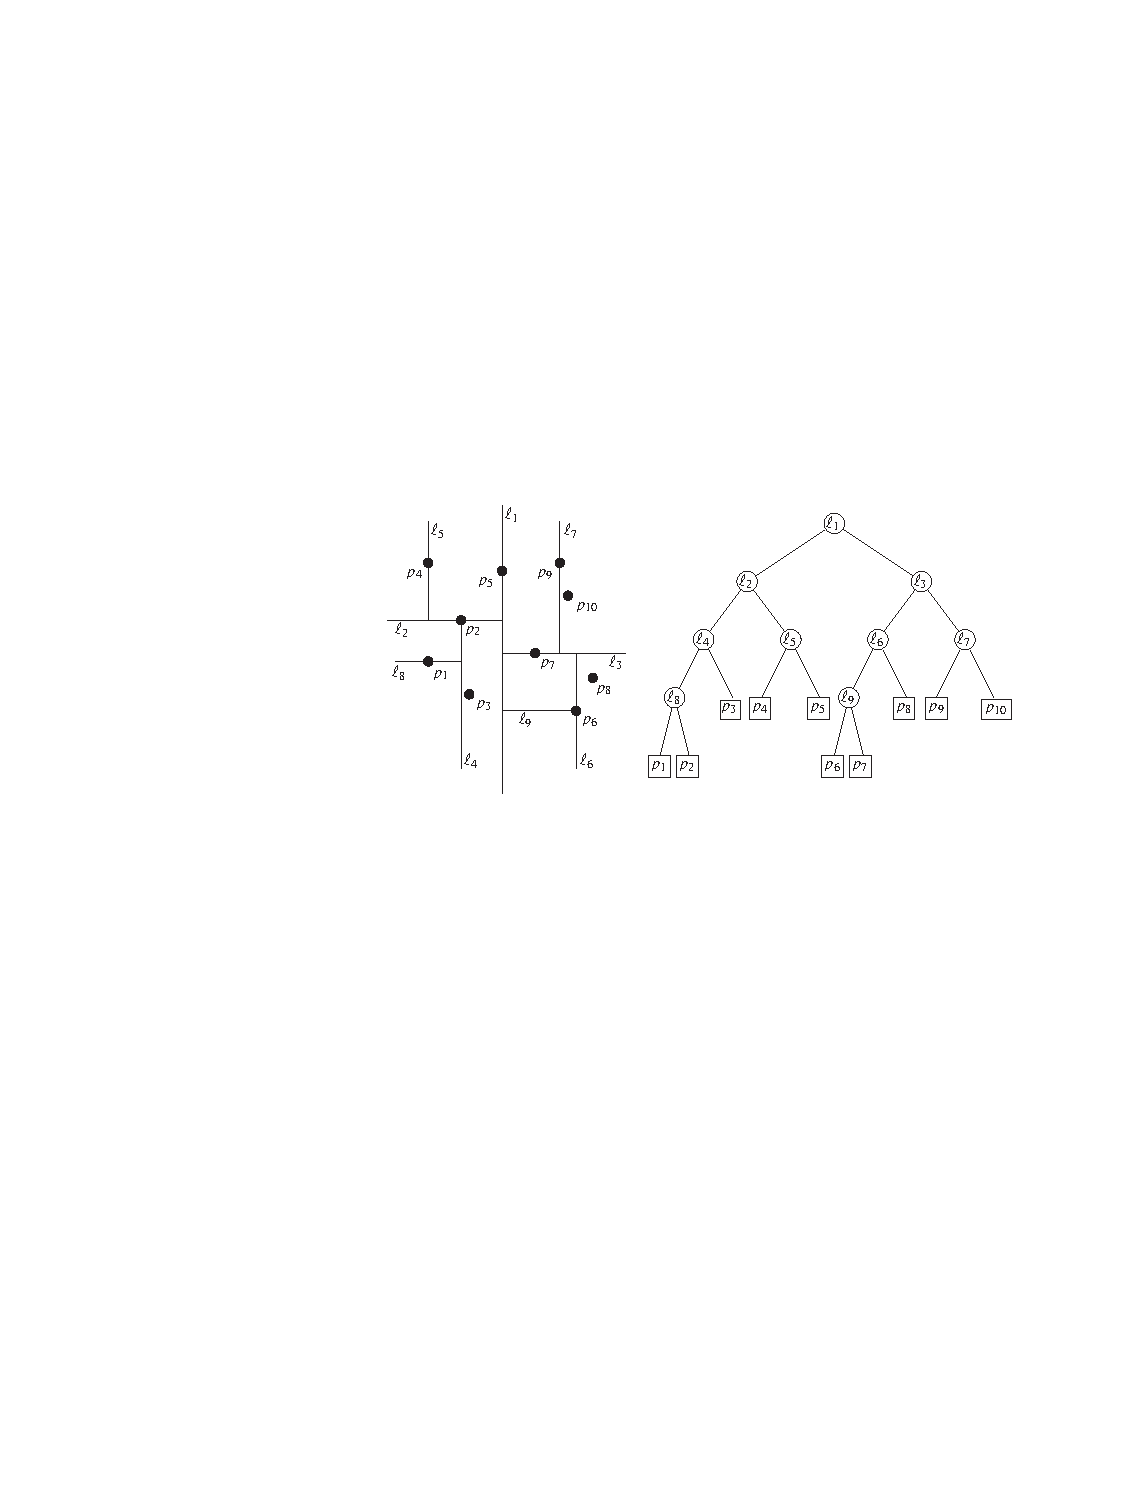
\includegraphics[width = 0.9 \textwidth]{figures/illustrations/kdtree.pdf}
    \caption{Exemplarische Darstellung eines \textsc{k-d-trees} für $d=2$ Dimensionen. In der linkten Hälfte ist die graphische Interpretation der Aufteilung und in der rechten der Aufbau des entstehenden Baumes zu finden \cite{de2000computational}. Der in der $i$-ten Iteration bestimmte Median ist als $l_i$ eingetragen. An jeder Astgabelung werden die Elemente falls sie kleiner als der Median $l_i$ sind in den linken und ansonsten in den rechten Zweig einsortiert.}
    \label{fig:kdtree}
\end{figure}

\improvement{Add search path example to the graph?}

Der Suchvorgang besteht aus zwei Phasen. Zuerst wird die Aufbauphase des Baumes durchgeführt, bei der die Trainingsdaten einsortiert und damit ein Suchindex erzeugt wird. Anschließend folgt die Suchphase, bei der der zuvor erstellte Suchindex nach dem nächsten Nachbarn durchsucht wird.\\

In der Aufbauphase wird zuerst eine Dimensionen ausgewählt und der Median $l_i$ der Daten in dieser Dimension bestimmt. Dieser Wert bildet eine Trennlinie, anhand derer die Punkte in zwei Mengen unterteilt werden, die entweder nur größere oder nur kleinere Elemente bezogen auf jene Dimension beinhalten. Die beiden Mengen bilden die ersten Äste des Baumes. Nun wird dieser Schritt rekursiv auf alle Äste angewendet, und die hierbei zum Vergleich genutzte Dimension iteriert \cite{de2000computational}. Dieses Verfahren wird so lange wiederholt, bis eine bestimmte maximale Anzahl $N_{max}$ an Knotenpunkten pro Ast erreicht wird. Ab dieser unteren Grenze wird das Erstellen des Binärbaumes beendet. Ab dieser Grenze benötigt der Zugriff auf die verschiedenen Elemente und das Aufteilen in neue Äste mehr Zeit, als das Berechnen der Abstände zwischen den verbleibenden $N_{max}$ Knoten und dem Suchpunkt. Eine beispielhafte Darstellung des Verfahrens ist in Abbildung \ref{fig:kdtree} zu finden.

Die Suchphase wird nun wieder rekursiv durchgeführt. Hierbei werden wieder iterierend die verschiedenen Dimensionen verglichen, und sich somit immer weiter im Suchbaum nach unten ein Weg gebahnt \cite{de2000computational}. In der untersten Ebene, also wenn nur noch eine Suche zwischen maximal $N_{max}$ Elemente durchgeführt werden muss, wird nun die \textit{brute force}-Suche genutzt. In dieser Arbeit ist für alle Anwendungen diese Schwelle auf $N_{max} = 40$ gesetzt worden \citep{scikitlearnneighbours}.\\

Diese Methode zeichnet sich durch eine Laufzeit aus, welche sich für einen einzelnen Suchvorgang wie $\mathcal{O}(\log(N))$ verhält \cite{bentley1975multidimensional}. Wird die Vorhersage für $m$ Datenpunkte durchgeführt ergibt sich die Laufzeit zu $\mathcal{O}(m\log(N))$. Dies ist geringer, als die Laufzeit eines naiven Suchvorgangs, welche sich wie $\mathcal{O}(mN)$ verhält. Zusätzlich muss bei der Verwendung des \textsc{k-d-tree}s allerdings auch noch die Baumstruktur aufgebaut werden. Hierfür besteht eine ungefähre Laufzeit $\mathcal{O}(N \log(N))$. Zusätzlich besitzt die Laufzeit des \textsc{k-d-tree}s auch eine Abhängigkeit von der Dimensionalität $d$. Es hat sich gezeigt, dass wenn $d$ hinreichend groß ist, die Vorteile geringer werden, und für hohe Dimensionalitäten ($\approx d > 20)$ die Suche ineffizient abläuft \citep{scikitlearnneighbours}.\\


\subsection{Radiale Basisfunktionen}
Eine weitere Methode um einen funktionalen Zusammenhang $F : X \rightarrow Y$ zu finden, welcher Daten der Menge $X \in \mathbb{R}^n$ auf Elemente aus $Y \in \mathbb{R}^m$ eindeutig abbildet, bieten die \textit{radialen Basisfunktionen} (im Folgenden als \textsc{RBF} abgekürzt) an. Auch dafür werden Daten benötigt, anhand derer der Zusammenhang erlernt werden kann. Diese Trainingsdaten sollen im Folgenden aus $N$ Datenpunkten bestehen.\\

Bei diesem Ansatz wird die gesuchte Funktion $F$ als Linearkombination aus vielen radialen Funktionen approximiert. Dafür werden $l$ Elemente $\{\vec{x}_i\}, i=1,...,l$ aus den Trainingsdaten ausgewählt und diese als so genannte \textit{Zentren} $\{\vec{z}_i\}$ genutzt. Hiermit lassen sich die Funktionen als $\phi_i(\vec{x}) = \phi(||\vec{x}-\vec{z}_i||), i=1,\ldots ,l$ darstellen \citep{lowe2multi}. Eine mögliche Wahl der Basisfunktionen sind zum Beispiel Gaußfunktionen
\begin{align*}
\phi_i(\vec{x}) = \exp \left( - \frac{||\vec{x}-\vec{z}_i||}{\sigma_{RBF, i}^2} \right),
\end{align*}
wobei $\sigma_{RBF, i}$ für die Breite der $i$-ten Gaußfunktion steht.
Die Linearkombination führt zu dem Ansatz 
\begin{align}
\label{eq:rbf_lincomb}
\vec{y} = F(\vec{x}) = \sum^l_{i=1} \vec{\omega}_i \phi(||\vec{x} - \vec{z}_i||).
\end{align}
Die $\vec{\omega}_i \in \mathbb{R}^m$ stehen hier für die \textit{Gewichtsvektoren} der einzelnen Basisfunktionen $\phi_i$ im Rahmen der Linearkombination.\\

Das Ziel besteht jetzt darin, die Gewichtsvektoren $\vec{\omega_i}$ approximativ zu bestimmen. Dafür werden zunächst drei Matrizen definiert, durch die das Problem ausgedrückt werden kann.\\
Die Matrix $\mathbf{Y} \in \mathbb{R}^{N \times m}$ repräsentiert die Funktionswerte der Abbildung und beinhaltet als Zeilen die $N$ verschiedenen Funktionswerte $\vec{y}_i$ der Trainingsdaten
\begin{align}
\mathbf{Y} \defeq
\begin{pmatrix}
y_{11} & \ldots  & y_{1m} \\
\vdots & & \vdots \\
y_{N1} & \ldots  & y_{Nm} \\
\end{pmatrix}.
\end{align}
Die Matrix $\mathbf{\Omega} \in \mathbb{R}^{l \times m}$ beinhaltet dagegen als Zeilen die Gewichtsvektoren
\begin{align}
\mathbf{\Omega} \defeq
\begin{pmatrix}
\omega_{11} & \ldots  & \omega_{1m} \\
\vdots & & \vdots \\
\omega_{l1} & \ldots  & \omega_{lm} \\
\end{pmatrix}.
\end{align}
Die dritte Matrix $\mathbf{A} \in \mathbb{R}^{N \times m}$ repräsentiert Anwendungen der radialen Basisfunktionen auf die Trainingsdaten 
\begin{align}
\mathbf{A} \defeq
\begin{pmatrix}
A_{11} & \ldots  & A_{1m} \\
\vdots & & \vdots \\
A_{N1} & \ldots  & A_{Nm} \\
\end{pmatrix},
\end{align}
wobei die einzelnen Elemente als $A_{ij} \defeq \phi(|| \vec{x}_i - \vec{y}_j ||)$ definiert sind.\\
Das Problem lässt sich somit durch
\begin{align}
\mathbf{Y} = \mathbf{A} \cdot \mathbf{\Omega}
\end{align}
ausdrücken \citep{lowe2multi}. Da die Matrizen $\mathbf{Y}$ und $\mathbf{A}$ konstruiert sind, besteht die Aufgabe lediglich darin die Matrix $\mathbf{\Omega}$ der Gewichte zu ermitteln. Der naheliegende Ansatz, das direkte Ermitteln der Inversen $\mathbf{A}^{-1}$ stellt sich dafür aus ungeeignet heraus, da das Problem meistens überkonditioniert ist und die Matrix nicht quadratisch ist, wodurch keine Inverse gefunden werden kann. Stattdessen ist es geschickter, das Problem als eine lineare Optimierungsaufgabe zu betrachten, bei der der Fehler $||\mathbf{A} \vec{\omega_i} - \vec{y}_i||^2$ minimiert werden soll.\\
Durch die Verwendung der \textit{Moore-Penrose Pseudoinversen} $\mathbf{A}'$ wird zugleich gewährleistet, dass die Lösung ausgewählt wird, die zudem auch die kleinsten Gewichte besitzt. Dies hilft den Effekt des \textit{Overfittings} zu verringern \cite{lowe2multi}. Das \textit{Overfitting} beschreibt den Effekt, dass das Vorhersage-Modell zu stark auf die Trainingsdaten angepasst ist, und das Verhalten nicht stark genug generalisiert. Dies ist an einem (deutlich) höheren Test- als Trainingsfehler zu erkennen.\\

Mit diesem Ansatz ergibt sich die Lösung zu
\begin{align}
\mathbf{\Omega} = \mathbf{A}' \cdot \mathbf{Y}.
\end{align}

Um nun Funktionswerte vorherzusagen, wird der oben eingeführte Zusammenhang \ref{eq:rbf_lincomb} zwischen den zuvor ermittelten Gewichten und der Zielvariable $\vec{y}$ genutzt.
\section{Neuronale Netzwerke}
%\subsection{Überblick über Neural Networks}
In den letzten Jahren hat die Technik der Neuronalen Netzwerke (Neural Networks) erneut stark an Popularität gewonnen. Dies liegt zum einen an der gestiegenen verfügbaren Rechenleistung und zum anderen an der Entwicklung hierfür notwendiger Algorithmen.\\
Allgemein lassen sich diese Netze in zwei große Gruppen aufteilen: die der \textsc{Feed Forward Neural Networks} und die der \textsc{Recurrent Neural Networks}, welche im Folgenden als \textsc{FFNN} respektive \textsc{RNN} bezeichnet werden.\\

Ein \textsc{FFNN} besteht aus mehreren Ebenen, welche jeweils aus verschiedenen nicht-linearen Einheiten zusammengesetzt sind. Die erste dieser Ebenen wird zur Eingabe und die letzte zur Ausgabe eines Signals genutzt. Eine Schematische Darstellung ist im linken Teil der Abbildung \ref{fig:ffnn_rnn_structure} zu finden. Die Einheiten zweier benachbarter Ebenen sind mit individuellen Gewichten vollständig in Richtung der Ausgabe verbunden. Dies bedeutet, dass jedes Einheit $x^n_i$ sein Signal an alle Einheiten der folgenden Ebene $x^{n+1}_j$ mit einem individuellen Gewicht $w^n_{i \rightarrow j}$ weitergibt. Zwischen den Einheiten innerhalb einer Ebene bestehen keinerlei Verbindungen.\\
Damit ein solches Netzwerk Vorhersagen treffen kann, müssen die Gewichte in einem Trainingsvorgang angepasst werden. Dies wird durch den \textsc{Backpropagation}-Algorithmus erreicht. Dabei wird eine Kostenfunktion $L$ minimiert. Dies wird erreicht, indem die Gewichte des Netzwerkes immer in die entgegengesetze Richtung des Gradienten $\nabla_w L$ angepasst werden, wodurch versucht wird ein Minimum der zu $L$ gehörigen Kostenlandschaft zu erreichen \cite{bishop}. Solche \textsc{FFNN} eigenen sich besonders gut zur Lösung von Klassifizierungsproblemen.\\

\begin{figure}[H]
    \centering
    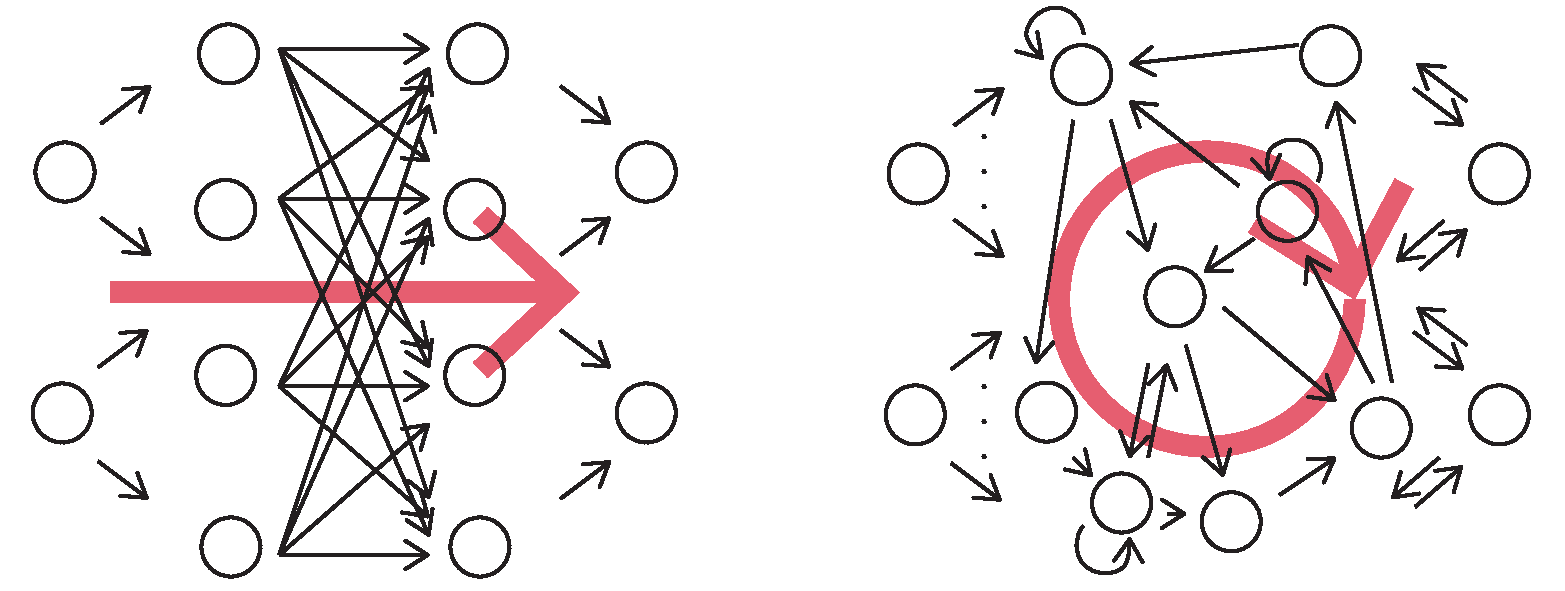
\includegraphics[width = 0.9 \textwidth]{figures/illustrations/ffnn_rnn_structure.pdf}
    \caption{Schematische Darstellung eines \textsc{FFNN} mit vier Ebenen (links) und eines \textsc{RNN} (rechts) mit ihren jeweiligen Verbindungen und der Eingangs- und Ausgangsebene. Der Informationsfluss ist in rot eingetragen (nach \citep{jeagerTut2002}).}
    \label{fig:ffnn_rnn_structure}
\end{figure}

Ein \textsc{RNN} hat einen ähnlichen Aufbau, doch hier können alle Einheiten an alle anderen Einheiten Signale weitergeben und von diesen erhalten. Die schematische Struktur ist im rechten Teil der Abbildung \ref{fig:ffnn_rnn_structure} dargestellt. Hierdurch erhält das Netzwerk eine Art Gedächtnisfunktion, wodurch temporale Strukturen verarbeitet und berücksichtigt werden können. Dies kann die Vorhersage in bestimmten Anwendungsbeispielen wie der Text- und Sprachanalyse verbessern.\\
Ein Nachteil ist, dass zum Trainieren, aufgrund der rekurrenten Struktur, nicht mehr der einfachere \textsc{Backpropagation}-Algorithmus genutzt werden kann, sondern eine für \textsc{RNN}s abgewandelte Form genutzt werden muss. Für den prominenteste Algorithmus werden die verschiedenen Zustände die das \textsc{RNN} im Laufe der Signal-Propagation annimmt nacheinander betrachtet und auf diese zeitliche Entwicklung anschließend der \textsc{Backpropagation}-Algorithmus angewendet. Diese Methode ist unter dem Namen \textsc{Backpropagation through Time} (BTT) bekannt. Sie ist zum einen rechenaufwendiger und zum anderen auch instabiler, da das Verschwindenden und auch das Explodieren des Gradienten der Kostenfunktion deutlich wahrscheinlicher als bei der gewöhnlichen \textsc{Backpropagation} ist \citep{pascanu, jeagerTut2002}. Da bei diesem Ansatz die Gewichte ebenfalls anhand des Gradienten der Kostenfunktion angepasst werden, wird der Algorithmus instabil, falls diese explodieren oder ineffizient, wenn sie verschwinden.

\section{Echo State Network}
\label{sc:esn}
\subsection{Überblick}
Um die (Leistungs)Probleme der \textsc{RNN} zu umgehen, wurden als mögliche Lösung die \textsc{Echo State Networks} von H. Jäger vorgeschlagen \cite{jaeger2010}. Etwa zeitgleich wurde von W. Maas das Modell der \textit{Liquid State Machines} vorgeschlagen. In diesem Modell steht der biologische Hintergrund im Fokus, doch sind die Ergebnisse denen der \textsc{Echo State Networks} sehr ähnlich \citep{Maass2011}. 

\subsection{Aufbau}
\label{sec:esn_structure}
Ein \textsc{ESN} ist eine Spezialform eines \textsc{RNN}s. Hierbei wird eine auf dem ersten Blick eigenartige Entscheidung getroffen: Während des gesamten Trainingsvorganges werden die Verbindungen der einzelnen Einheiten größtenteils nicht verändert. Es wird versucht durch das \textit{Echo} der vorherigen Signale, welche noch im Netzwerk gespeichert sind, diese Signale zu rekonstruieren - hieraus ergibt sich auch der Name \cite{lukoseviciusa2009}. Im Folgenden wird der Aufbau und anschließend die Funktionsweise eines solchen Netzwerkes nach \citep{jaeger2007} beschrieben.\\

Allgemein bildet das Netzwerk $S$ ein zeitliches Signal $\vec{u}(n) \in \mathbb{R}^{N_u}$  auf eine zeitlich variable Ausgabe $\vec{y}(n) \in \mathbb{R}^{N_y}$ für die Zeiten $n=1, ..., T$ ab. Zudem besitzt das System ein sogenanntes \textsc{Reservoir} aus $N$ nicht-linearen Einheiten. Der innere Zustand des Netzwerkes wird durch diese Einheiten beschrieben und als $s(n) \in \mathbb{R}^{N}$ bezeichnet.\\
Die Verbindungen der inneren Einheiten untereinander werden durch die Gewichtsmatrix $\mathbf{W} \in \mathbb{R}^{N \times N}$ beschrieben. Das Eingangssignal wird zusammen mit einem \textit{Bias} $b_{in} \in \mathbb{R}$ durch die Matrix $\mathbf{W_{in}} \in \mathbb{R}^{N \times (N_u+1)}$ auf die inneren Einheiten weitergeleitet.\\

Die zeitliche Entwicklung der inneren Zustände berechnet sich nach der Vorschrift
\begin{align}
\label{eq:esn_stateeq}
\vec{s}(n) = (1 - \alpha) \cdot \vec{x}(n-1)  + \alpha \cdot f_{in}\left( \mathbf{W_{in}} [b_{in}; \vec{u}(n)] + \mathbf{W} \vec{x}(n-1) \right),
\end{align}
wobei $f_{in}$ eine beliebige (meistens \textit{sigmoid}-förmige) Transferfunktion ist, und $[\cdot\,;\,\cdot]$ das vertikale Aneinanderfügen von Vektoren beziehungsweise Matrizen bezeichnet. Für diese Zustandsgleichung wurde das Modell eines \textit{Leaky Integrator Neurons} genutzt, wobei $\alpha \in (0,1]$ die Verlustrate beschreibt. Für $\alpha=1$ ergibt sich als Spezialfall ein gewöhnliches Neuron
\begin{align}
\vec{s}(n) = f_{in}\left( \mathbf{W_{in}} [b_{in}; \vec{u}(n)] + \mathbf{W} \vec{x}(n-1) \right).
\end{align}

Da für manche Anwendungsfälle auch eine direkte Rückkopplung wünschenswert ist, kann das System noch um eine Ausgabe-Rückkopplung erweitert werden. Diese verbindet die Ausgabe erneut mit den inneren Einheiten durch die Matrix $\mathbf{W_{fb}} \in \mathbb{R}^{N \times N_y}$.
Somit ergibt sich 
\begin{align}
\label{eq:esn_stateeq_feedback}
\vec{s}(n) = (1 - \alpha) \cdot \vec{x}(n-1)  \alpha \cdot f_{in}\left( \mathbf{W_{in}} [b_{in}; \vec{u}(n)] + \mathbf{W} \vec{x}(n-1) + \mathbf{W_{fb}} \vec{y}(n) \right)
\end{align}
als Zustandsgleichung. In Abbildung \ref{fig:esn_structure} ist der vollständige Struktur eines \textsc{ESN}s mit den Matrizen $\mathbf{W_{in}}, \mathbf{W}$ und $\mathbf{W_{out}}$ dargestellt.

\begin{figure}[H]
    \centering
    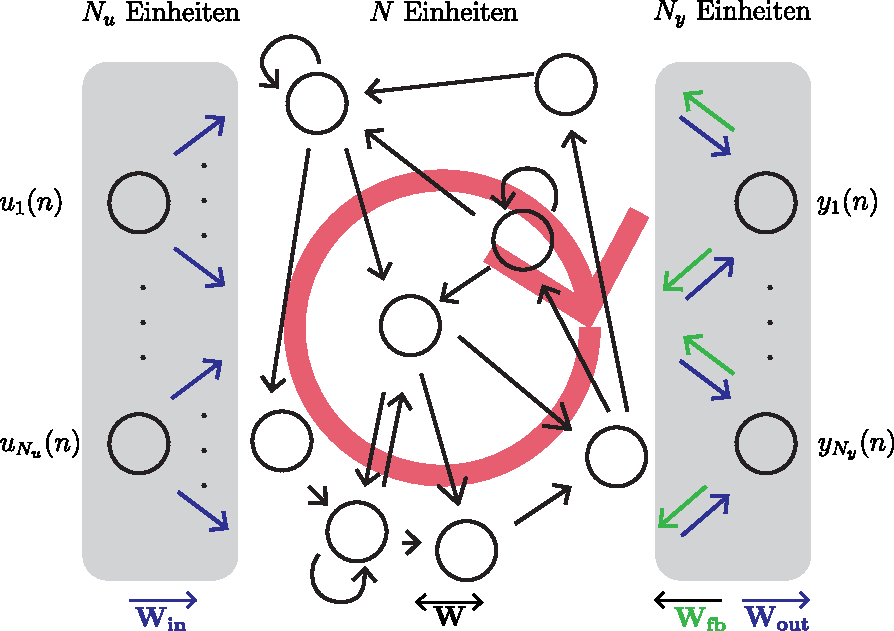
\includegraphics[width = 0.7 \textwidth]{figures/illustrations/esn_structure.pdf}
    \caption{Schematische Darstellung eines \textsc{ESN}. Von links nach rechts durchläuft das Eingangssignal $u(n)$ erst $N_u$ Eingangseinheiten, danach ein Reservoir mit $N$ Einheiten, bis schließlich die Ausgabe $y(n)$ mittels $N_y$ Ausgabeeinheiten gebildet wird. (nach \citep{jeagerTut2002, Ma2013}).}
    \label{fig:esn_structure}
\end{figure}


Anhand der inneren Zustände lassen sich nun noch die sogenannten erweiterten inneren Zustände $x(n) = [b_{out}; \vec{s}(n); \vec{u}(n)] \in \mathbb{R}^{1 + N_u + N}$ definieren, wobei $b_{out}$ ein \textit{Bias} für die Ausgabe darstellt. 

Aus diesen erweiterten inneren Zuständen kann nun die Ausgabe $\vec{y}(n)$ konstruiert werden. Dies kann entweder im Sinne einer Linearkombination durch die Ausgangsmatrix $\mathbf{W_{out}} \in \mathbb{R}^{(1 + N_u + N) \times N_y}$ oder durch andere nicht lineare Regressionsalgorithmen wie beispielsweise einer \textsc{Support Vector Machine (SVM)} durchgeführt werden. Im Folgenden wird nur der Fall einer Linearkombination betrachtet, da sich für die anderen Methoden ein analoges Verfahren ergibt.
In diesem Fall berechnet sich die Ausgabe mittels
\begin{align}
\vec{y}(n) = f_{out} \left( \mathbf{W_{out}} \vec{x}(n) = \mathbf{W_{out}} [b_{out}; \vec{s}(n); \vec{u}(n)] \right),
\end{align}
wobei $f_{out}$ die Transferfunktion der Ausgabe ist. Für diese kann in den meisten Fällen (so auch in dieser Arbeit) die Identität $f_{out}(x) = x$ genutzt werden.\\

Während die Matrix $\mathbf{W_{out}}$ durch den Trainingsvorgang bestimmt wird, werden die Matrizen $\mathbf{W_{in}}$ und $\mathbf{W}$ a priori generiert und festgelegt. Hierbei hat sich für das Generieren der Eingangsmatrix eine zufällige Anordnung von zufälligen Gleitkommazahlen zwischen $-0.5$ und $0.5$ als geschickt herausgestellt. Falls ein Feedback gewünscht ist, also Gleichung (\ref{eq:esn_stateeq_feedback}) genutzt wird, wird $\mathbf{W_{fb}}$ gleichartig konstruiert. Auf das Generieren der inneren Matrix $\mathbf{W}$ wird in Abschnitt \ref{sc:esn_theory} genauer eingegangen.

\subsection{Trainingsvorgang}
Nachdem der Aufbau des Netzwerkes beschrieben ist, ergibt sich nun die Frage, wie der Trainingsvorgang durchgeführt wird.

Hierfür wird für die Zeiten $n=0, ..., T_0$ das \textsc{ESN} mit dem Signal $\vec{u}(n)$ betrieben, wobei $T_0$ die \textit{transiente Zeit} beschreibt. Hierdurch soll das System aus seinem zufällig gewähltem Anfangszustand in einen charakteristischen Zustand übergehen. Anschließend wird das System für Zeiten $n < T$ weiter betrieben und die erweiterten Zustände $\vec{x}(n)$ als Spalten in der \textit{Zustandsmatrix} $\mathbf{X} \in \mathbb{R}^{(1 + N_u + N) \times T}$ gesammelt. Analog dazu werden die gewünschten Ausgaben $\vec{y}(n)$ nach dem Anwenden der Inversen $f^{-1}_{out}$ der Ausgabe-Transferfunktion $f_{out}$ auch als Spalten in der \textit{Ausgabematrix} $Y \in \mathbb{R}^{N_y \times T}$ gesammelt.
Nun wird eine Lösung der Gleichung
\begin{align}
\mathbf{Y} = \mathbf{W}_{out} \mathbf{X}
\end{align}
für $\mathbf{W}_{out}$ gesucht. Hierfür stehen mehrere Verfahren zur Verfügung, von denen zwei prominente erwähnt sein sollen.
Zum einen kann die Lösung durch eine \textit{Tikhonov Regularisierung} mittels der Regularisierung $\beta \cdot ||\vec{W}_{out, i}||^2$ der Gewichtsmatrix mit der Konstante $\beta$ erhalten werden. Hierbei steht $\vec{W}_{out, i}$ für die jeweils $i$-te Zeile der Gewichtsmatrix. Das Verfahren
\begin{align}
\label{eq:tikhonov}
\mathbf{W}_{out} = \mathbf{Y} \mathbf{X}^T \left(\mathbf{X} \mathbf{X}^T + \beta I \right)^{-1}
\end{align}
ist sehr leistungsstark, aber auch teilweise numerisch instabil. Bei geeigneter Wahl von $\beta$ können die besten Ergebnisse hinsichtlich der Genauigkeit der Vorsage erzielt werden \cite{lukoseviciusa2009}. Deshalb wird in dieser Arbeit auch nur dieses Lösungsverfahren verwendet. Die weiteren Lösungsansätze für das Gleichungssystem sind nur aus Gründen der Vollständigkeit angegeben.\\

Zum anderen kann zur Lösung die \textit{Moore-Penrose-Pseudoinverse} $\mathbf{X}'$ genutzt werden, sodass für die Ausgabematrix
\begin{align}
\label{eq:pseudo_inverse}
\mathbf{W}_{out} = \mathbf{Y} \mathbf{X}'
\end{align}
folgt. Dieses Verfahren ist zwar sehr rechenaufwendig aber dafür numerisch stabil \cite{lukoseviciusa2009, jaeger2012}. Nichts desto trotz, kann allerdings auf Grund des Fehlens einer Regularisierung leicht der Effekt des \textsc{Overfittings} auftreten. Auf Grund dessen wird es in dieser Arbeit nicht verwendet.\\

Um den Effekt des Overfittings bei der Verwendung der Psuedoinversen zu reduzieren, kann in der Zustandsgleichung (\ref{eq:esn_stateeq}) beziehungsweise (\ref{eq:esn_stateeq_feedback}) eine leichte normalverteilte Störung $\vec{\nu}(n)$ der Größenordnung $\num{1e-1}$ bis $\num{1e-5}$ addiert wird. Falls die \textit{Tikhonov Regularisierung} zur Lösung verwendet wird, erhöht die Verwendung der zufälligen Störung die Stabilität der Vorhersage des System. Dieser Ansatz beruht auf Empirie, da eine mathematische Begründung hierfür noch nicht vollständig gelungen ist \citep{jaeger2010, lukoseviciusa2009}. Anschaulich lässt sich das Vorgehen dadurch motivieren, dass hierdurch künstliche Datenpunkte in der nähe der vorhandenen Trainingsdaten emuliert werden, und somit eine größere Vielfalt an Daten während der Trainingsphase beobachtet wird.\\

Zusammenfassend ergibt sich somit der folgende Funktionsablauf für die Anwendung eines \textsc{ESN}:

\singlespacing
\begin{enumerate}
	\item Zufälliges Generieren der Matrizen $\mathbf{W}_{in}, \mathbf{W}_{fb}$ und Konstruktion der Matrix $\mathbf{W}$ 
	\item Einspeisen des Signals $u(n)$ und Konstruktion der Zustandsmatrix $\mathbf{X}$ und der Ausgabematrix $\mathbf{Y}$ 
	\item Berechnung der Ausgabematrix $\mathbf{W}_{out}$
	\item Einspeisen des Signals $u(n)$ für Vorhersagen des Signales $y(n)$ für $n > T$
\end{enumerate}
\onehalfspacing

Zusätzlich zu diesen Eigenschaften wird die Dynamik des Reservoirs auch von dessen Größe $N$ bestimmt. Es kann gezeigt werden, dass die Gedächtnisleistung eines Reservoirs stark von dieser abhängt. Somit ist es ratsam für Aufgaben, die eine lange Gedächtnisleistung benötigen, ein großes und für Aufgaben, die nur ein Kurzzeitgedächtnis benötigten, ein kleines Reservoir zu benutzen \citep{jeagerTut2002}.





\subsection{Theoretischer Hintergrund}
\label{sc:esn_theory}
Um die mathematischen Eigenschaften beschreiben zu können, sind zuerst zwei Definitionen nötig \cite{yildiz}.

\begin{definition}[Kompatibler Zustand]
Sei $S : X \times U \rightarrow X$ ein \textsc{ESN} mit der Zustandsgleichung $\vec{x}_{n+1} = F \left( \vec{x}_n, \vec{u}_{n+1} \right)$. Eine Folge von Zuständen $(\vec{x}_n)_n$ ist kompatibel mit der Eingangsfolge $(\vec{u}_n)_n$, wenn $\vec{x}_{n+1} = F\left( \vec{x}_n, \vec{u}_{n+1} \right), \forall n \leq 0$ erfüllt ist.
\end{definition}

\begin{definition}[Echo State Eigenschaft (ESP)]
Ein \textsc{ESN} $S : X \times U \rightarrow X$ besitzt die \textit{Echo State Eigenschaft} genau dann wenn eine Nullfolge $(\delta_n)_{n \geq 0}$ existiert, sodass für alle Zustandsfolgen $(\vec{x}_n)_n, (\vec{x}'_n)_n$ die kompatibel mit der Eingangsfolge $(\vec{u}_n)_n$ sind gilt, dass $\forall n \geq 0 ||x_n - x'_n|| < \delta_n$
\end{definition} 
Dies bedeutet, dass nachdem das Netzwerk lang genug betrieben worden ist, der Zustand nicht mehr von dem beliebig gewähltem Anfangszustand abhängt. Diese Eigenschaft ist notwendig, damit das \textsc{ESN} Vorhersagen treffen kann \cite{jeagerTut2002}.\\

Nun stellt sich die Frage, wann ein Netzwerk diese Eigenschaft besitzt. Es wird schnell klar, dass dies hauptsächlich durch die Gewichtsmatrix $\mathbf{W}$ bestimmt wird. Betrachtet man die Zustandsgleichung des Netzwerkes, so lässt sich auf Grund des \textit{Banachschen Fixpunktsatzes} erkennen, dass die \textit{ESP} für alle Eingänge $\vec{u}_n$ vorliegt, sobald $||\vec{x}_{n+1} - \vec{x}'_{n+1}|| < ||\vec{x}_n - \vec{x}'_n||$ für zwei kompatible Zustände $\vec{x}_n \neq \vec{x}'_n$ erfüllt ist \cite{jaeger2010}.
Hieraus ergibt sich, dass die \textit{ESP} vorliegt, wenn 
\begin{align}
\label{eq:theory_old_requirement}
|1-\alpha(1-\sigma_{max}(\mathbf{W}))| < 1
\end{align}
erfüllt ist, wobei $\sigma_{max}(\mathbf{W})$ der größte Singulärwert ist \cite{jaeger2007}.\\
Weitergehend ist bekannt, dass für Systeme bei denen der Spektralradius $\rho(\mathbf{W}) > 1$ ist diese Eigenschaft nicht vorliegen kann, sofern $\vec{u}_n = 0$ möglich ist \cite{jaeger2007, jaeger2010}.\\

Hieraus ergab sich lange Zeit die falsche Annahme, dass für Systeme mit $\rho(\mathbf{W}) < 1$ die Eigenschaft stets garantiert ist. Wie allerdings gezeigt werden konnte, ist dies nicht der Fall \citep{yildiz}. Stattdessen konnte gezeigt werden, dass eine hinreichende Bedingung durch
\begin{align}
\label{eq:theory_sufficient_requirement}
\rho(\alpha |\mathbf{W}|+(1-\alpha) \mathbf{I}) < 1
\end{align}
gegeben ist - wobei als Betrag der Matrix hier das elementweise Betragsnehmen gemeint ist. Diese Bedingung ist weniger einschränkend als Gleichung (\ref{eq:theory_old_requirement}) \cite{yildiz}.\\

Weitergehend hat sich in Experimenten gezeigt, dass eine dünnbesetze Gewichtsmatrix $\mathbf{W}$ zu reicheren Dynamiken innerhalb des Reservoirs führen kann \citep{jaeger2010}. Eine solche dünnbesetze Matrix bedeutet, dass nicht mehr jedes Neuron mit jedem anderen Neuron verbunden ist, sondern dass nur noch ein relativer Anteil $\epsilon$ dieser Verbindungen vorhanden ist. Da durch eine größere Anzahl an verschiedenen internen Dynamiken vielfältigere Funktionen besser approximiert werden können, kann die Vorhersagequalität durch einen Geringen $\epsilon$ Wert erhöht werden.\\

Darauf basierend kann nun eine Methode nach \cite{yildiz} angegeben werden, um die Gewichtsmatrix $\mathbf{W}$ zu konstruieren:

\singlespacing
\begin{enumerate}
	\item Generiere zufällige Matrix $\mathbf{W}$ mit $\mathbf{|W|} = \mathbf{W}$ bei der in jeder Zeile nur $\epsilon$ Einträge ungleich $0$ sind.
	\item Skaliere $\mathbf{W}$, sodass Gleichung (\ref{eq:theory_sufficient_requirement}) erfüllt ist.
	\item Wechsel zufällig das Vorzeichen von ungefähr der Hälfte aller Einträge.
\end{enumerate}
\onehalfspacing

Statt dieser Vorschrift wurde zuvor oftmals $\mathbf{W}$ zufällig generiert und anschließend nur $\rho(\mathbf{W})$ statt $\rho(|\mathbf{W}|)$ skaliert, was mit unter zu instabilen Systemen geführt hat. Da allerdings auch für Systeme mit einem Spektralradius $ > 1$ die \textit{ESP} beobachtet werden kann für nicht verschwindende Eingänge $\vec{u}_n$, ist es ratsam auch effektive Spektralradien jenseits $1$ auszuprobieren.
\chapter{Anwendungen}

Die zuvor in Kapitel \ref{ch:theory} eingeführten Methoden werden nun durch drei verschiedene Szenarien ausprobiert und verglichen. Hierbei liegt der Fokus auf der Verwendung und Erprobung der \textsc{ESN}s. Da die klassischen Methoden der \textit{nächsten Nachbarn} (\textsc{NN}) und der \textit{radialen Basisfunktionen} (\textsc{RBF}) bereits seit längerer Zeit bekannt sind und populäre Lösung solcher Problemfälle darstellen, dienen sie als Bezugsgröße.\\

Jedes der drei Szenarien wird sowohl auf ein \textit{Barkley}-System als auch auf ein System nach dem \textit{Mitchell-Schaeffer}-Modell angewendet. Diese Systeme bestehen aus $150$ Gitterpunkten und nutzen die zuvor beschriebenen Parameter. Für ihre Startverteilung werden die Felder der beiden Systemvariablen in $100$ Quadrate unterteilt, und diese mit Zufallswerten zwischen $0$ und $1$ initialisiert. Anschließend werden die Systeme über $2000$ Zeitschritte ($\widehat{=} 400.0$ Zeiteinheiten) simuliert um ein transientes Verhalten abzuwarten. Durch das weitere Simulieren der Systeme werden die Test und Trainingsdaten ermittelt. Dabei wird für das \textit{Barkley} eine Samplingzeit von $0.1$ und für das \textit{Mitchell-Schaeffer}-Modell von $1.0$ Zeiteinheiten benutzt.\\
 
Die erste Aufgabe besteht darin aus der Kenntnis einer der beiden Systemvariablen die andere Unbekannte zu ermitteln. Dabei wird die Spannungsvariable als Quelle genutzt. Dies ist in den zuvor eingeführten Modellen jeweils die Größe, welche den Diffusionsterm beinhaltet; also die $u$-Variable im \textit{Barkley}-Modell und die $v$-Variable im \textit{Mitchell-Schaeffer}-Modell.\\
Im zweiten Szenario werden die Techniken verwendet um aus Messdaten einer simulierten Fernfeldmessung der Spannungsvariable  diese wiederherzustellen. Diese Fernfeldmessung wird durch eine gaußsche Unschärfe simuliert.\\
Abschließend wird die Spannungsvariable der inneren Punkte eines Quadrates nur durch die Kenntnis der Randwerte des Systems vorhergesagt.\\

\unsure{Add subchapter?}
\section{Allgemeines Vorgehen}
\label{sc:experiments_general}
Das Ziel aller drei Aufgaben besteht jeweils darin ein zweidimensionales Feld vorherzusagen. Eine naheliegende Möglichkeit dies zu schaffen besteht darin wirklich den gesamten Inhalt des $150 \times 150$ Einheiten großen Feldes auf einmal vorherzusagen. Da dabei die Ausgabe der Vorhersage aus einem $22500$-dimensionalen Vektor besteht werden sehr viele Trainingsdaten benötigt, um genügend Informationen über eine solch hochdimensionale Ausgabe zu erhalten. Um dieses Problem zu umgehen wird stattdessen ein Verfahren benutzt, bei dem jeder Punkt einzeln vorhergesagt wird. Dies hat zudem den Vorteil, dass aus einer monströsen Vorhersage, welche mitunter viel Arbeitsspeicher verbrauchen würde, in viele kleine Vorhersagen aufteilt. Hierdurch sinkt der zur Berechnung benötigte Bedarf an Arbeitsspeicher drastisch.\\

\begin{figure}[h]
\centering
\begin{subfigure}{.5\textwidth}
  \centering
  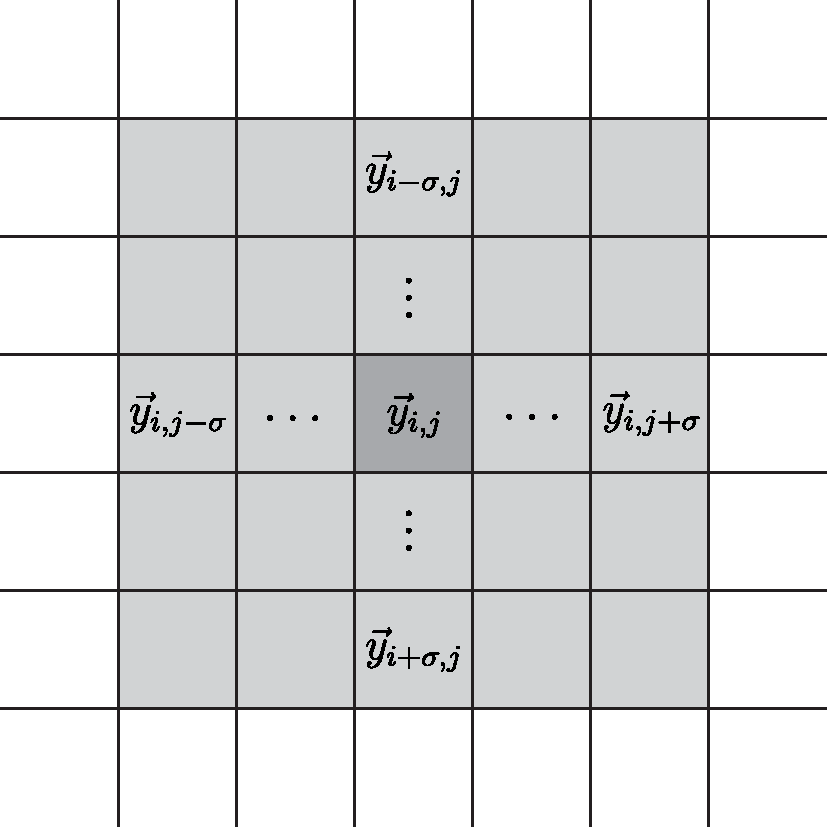
\includegraphics[width=.8\linewidth]{figures/illustrations/sigma_patches.pdf}
  \caption{Messsonde ohne Abstände zwischen\\den Messpunkten}
  \label{fig:probe_illustration_no_gaps}
\end{subfigure}%
\begin{subfigure}{.5\textwidth}
  \centering
  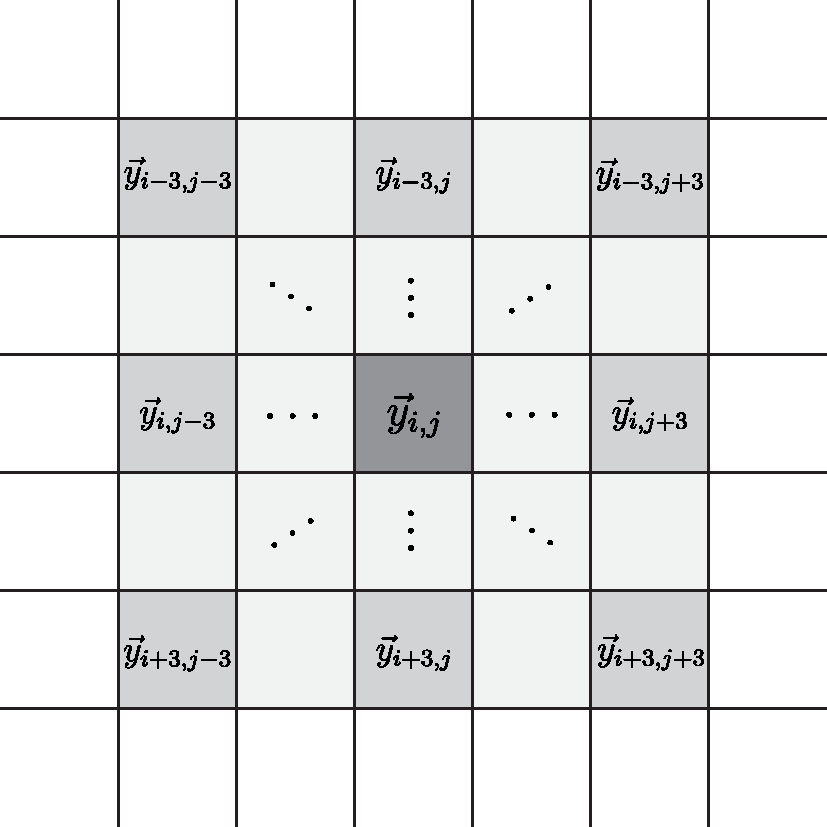
\includegraphics[width=.8\linewidth]{figures/illustrations/sigma_patches_gaps.pdf}
  \caption{Messonde mit einem Abstand von zwei Einheiten zwischen den Messpunkten}
  \label{fig:probe_illustration_gaps}
\end{subfigure}
\caption{Illustration der verwendeten \textit{Messsondentechnik}. Abbildung \ref{fig:probe_illustration_no_gaps} deutet an, wie aus einem $\sigma^2$ großem Quadrat um den eigentlichen Messpunkt Daten für die Vorhersage genutzt werden. Dagegen ist in Abbildung \ref{fig:probe_illustration_gaps} das Verfahren für $\sigma=5$ und $\Delta \sigma = 2$ dargestellt, sodass insgesamt die Information aus $9$ Punkten genutzt wird.}
\label{fig:probe_illustration}
\end{figure}

Des Weiteren kann angenommen werden, dass die Dynamiken einen ausgeprägten lokalen Charakter besitzen, sodass zumindest bei den ersten beiden Aufgaben weit entfernte Punkte keinen unmittelbaren Einfluss auf die Vorhersage haben. Darauf basierend kann eine sogenannte \textit{Messsondentechnik} entwickelt und für diese genutzt werden. Hierbei werden nicht nur die Informationen an einem Punkt $(i, j)$ für die Vorhersage, sondern auch die benachbarten Punkte, welche in einem Quadrat um $(i, j)$ liegen, genutzt. Eine Veranschaulichung ist in \ref{fig:probe_illustration_no_gaps} zu finden. Die Größe des Quadrates wird durch den Parameter $\sigma$ bestimmt, und ergibt sich zu $\sigma^2$. Da direkt Nachbarn unter Umständen durch den geringen Abstand sehr ähnliche Informationen beinhalten können, wird zudem ein Parameter $\Delta \sigma$ eingeführt, welche den Abstand zweier benachbarter Punkte, deren Information simultan verwendet werden, angibt. Eine beispielhafte Darstellung hiervon ist für $\sigma = 5, \Delta \sigma=2$ in Abbildung \ref{fig:probe_illustration_gaps} dargestellt. Dabei werden nur die Zeitreihen der Gitterpunkte genutzt, welche dunkelgrau hinterlegt sind, und die hellgrauen Informationen verworfen. Die Parameter, welche für die ersten beiden Aufgaben überprüft werden, sind in Tabelle \ref{tab:probe_sigma_values} aufgelistet. Dabei ist anzumerken, dass die Diskretisierung des Diffusionstermes in den Differentialgleichungen einem Wert $\sigma=3$ entsprechen würde.\\
Durch dieses Vorgehen kann für jeden Gitterpunkt ein ${\left \lceil{\frac{\sigma}{\Delta \sigma}}\right \rceil}^2$-dimensionaler Eingabevektor erstellt und für die ersten beiden Vorhersage-Aufgaben genutzt werden.\\

\begin{table}[h]
\centering
\begin{tabular}{c||c|c|c|c|c|c|c|}
$\sigma$ & 1 & 3 & \multicolumn{2}{c|}{5} & \multicolumn{3}{c|}{7} \\
\hline
$\Delta \sigma$ & 1 & 1 & 1 & 2 & 1 & 2 & 3 \\
\end{tabular} 
\caption{In den ersten beiden Aufgaben verwendete Parameter $\sigma$ und $\Delta \sigma$ für die \textit{Messsondentechnik}.}
\label{tab:probe_sigma_values}
\end{table} 

Der Trainingsvorgang wird jeweils über $N_{Training}=15000$ Zeitschritte durchgeführt und der Anschließende Evaluationsdurchgang auf $N_{Testing} = 2000$ Zeitschritte.
Zur Bewertung der Leistung einer Vorhersage werden die beiden Fehlergrößen MSE und NRMSE eingeführt. Im Allgemeinen ist der MSE (\textit{Mean Squared Error}) durch
\begin{align}
MSE(y) = \sum_i^m \sum_t^{N_{Testing}} \left(y(t)_i - \hat{y}(t)_i \right)^2
\end{align}
definiert und charakterisiert die Genauigkeit einer Vorhersage $\hat{y}$ im Vergleich zu dem tatsächlichen Wert $y \in \mathbb{R}^m$ über den Zeitraum $N_{Testing}$. Der NRMSE normiert diesen Fehler noch auf eine Vorhersage, bei der der Mittelwert $\langle y \rangle$ über die Trainingsphase als vorhergesagten Wert genutzt wird. Er ist als
\begin{align}
NRMSE(y) = \sqrt{\frac{MSE(y)}{MSE\left(\langle y \rangle\right)}}
\end{align}
definiert. Zusätzlich zu diesen Fehlermaßen werden im Folgenden oftmals auch die Laufzeiten der Ansätze angegeben. Hierbei ist zu beachten, dass diese nicht über mehrere Ausführungen des identischen Programmes gemittelt worden sind, und deshalb nicht als statistisch relevante Information sondern nur als ein Hinweis gesehen werden können.\\

Unter der Kenntnis, dass in den Modellen nur Werte zwischen $0$ und $1$ angenommen werden dürfen beziehungsweise angenommen werden, werden die Vorhersagen auf das Intervall $[0, 1]$ beschränkt. Dafür werden die Werte beider Variablen der Systeme sowohl nach unten als auch nach oben hin nach 
\begin{align}
x = \begin{cases}
	0,& \text{wenn } x \leq 0\\
	x,& \text{wenn } x \geq 0 \land \leq 1\\
    1,& \text{wenn } x \geq 1
\end{cases}
\end{align}
abgeschnitten, wobei $x$ für eine der beiden Variablen in dem jeweiligen Modell steht.

\FloatBarrier
\subsection{Echo State Network}
\label{sec:exp_general_esn}
\textit{Echo State Networks} besitzen viele verschiedene Hyperparameter, welche die Qualität der Vorhersage beeinflussen können. Dazu zählen nach \ref{sc:esn} die Reservoirgröße $N$, der Spektralradius $\rho$, die Verlustrate $\alpha$, die Amplitude der zufälligen Störung $\nu$, die Stärke der Regularisierung $\lambda$ und der Anteil der vorhandenen internen Verbindungen $\epsilon$. Da es zum aktuellen Zeitpunkt noch keinen zufriendenstellenden mathematischen Algorithmus für das das selbstständige optimale Einstellen eines \textsc{ESN}s gibt, müssen die Parameter manuell ermittelt werden. Hierfür wird in dieser Arbeit eine \textsc{GridSearch} benutzt. Bei diesem Verfahren wird der Hyperparameterraum in festgelegten Schritten abgetastet und die Leistung des somit entstehenden Netzwerke evaluiert und somit die besten Parameter ermittelt. Durch die hohe Anzahl der einstellbaren Hyperparameter und die nicht zu vernachlässigende Rechenzeit für das Trainieren und Evaluieren eines Netzwerkes, ist es nicht sinnvoll diese Suche für alle Komponenten des hochdimensionalen Zielvektors gleichzeitig durchzuführen. Stattdessen wird zuerst unter der Annahme, dass die Dynamik sich lokal an allen Punkten ähnlich verhält, ein Punkt in der Mitte des Feldes ausgewählt, und nur versucht diesen einen einzelnen Punkt vorherzusagen. Diese Aufgabe kann deutlich schneller berechnet werden, sodass nun die optimalen Hyperparameter mit einer \textsc{GridSearch} gesucht werden können. Im Anschluss können die Hyperparameter des  zuvor ermittelten \textsc{ESN} für die Vorhersage aller Punkte genutzt werden. Abschließend wird noch einmal Versucht das gefundene Reservoir manuell zu verbessern, indem die Parameter $N$ und $\lambda$ noch einmal variiert werden.\\
Es ist zu erwarten, dass die hierbei gefundenen Hyperparameter eine akzeptable Leistung für die jeweiligen Probleme erzielen können. Da allerdings bei dem zuvor beschriebenen Verfahren bei weitem nicht alle sinnvollen Hyperparameter getestet werden können, besteht die Möglichkeit, dass es noch besser geeignete Reservoirs mit anderen Hyperparametern gibt, welche eine noch höhere Leistung erzielen können.

\FloatBarrier
\subsection{Klassische Methoden}
Die klassischen Methoden sind nicht von alleine aus in der Lage zeitlich ausgeprägte Dynamiken vorherzusagen, da den Methoden a priori keine Informationen über die vorherigen Zustände vorliegen. Um dieses Problem zu lösen können Verzögerungs-Koordinaten mittels der in Abschnitt \ref{sc:delay_reconstruction} beschriebenen \textit{Delay Reconstruction} für die in Abschnitt \ref{sc:experiments_general} beschriebenen Vektoren aufgestellt werden. Die über die Autokorrelation ermittelte zeitliche Verzögerung $\tau$ ist für beide Systeme in Tabelle \ref{tab:delay_reconstruction_tau} dargestellt.     

\begin{table}[h]
\centering
\begin{tabular}{|c|c|}
$\tau_{Barkley}$ & $\tau_{Mitchell-Schaeffer}$ \\ 
\hline 
\hline 
0.64 Zeiteinheiten & 2.38 Zeiteinheiten\\ 
\hline 
\end{tabular} 
\caption{Verwendete zeitliche Verzögerung $\tau$ für die \textit{Delay Reconstruction} für das \textit{Mitchell-Schaeffer}- und das \textit{Barkley}-Modell}
\label{tab:delay_reconstruction_tau}
\end{table} 

\section{Kreuz-Prädiktion}
\label{sec:exp_cross_pred}
Momentan ist es durch invitro Experimente bereits möglich die Ausbreitung der elektrischen Erregung auf der Oberfläche des Herzmuskels experimentell aufzuzeichnen. Nun stellt sich die Frage, ob anhand beispielsweise der Messung der Membramspannung weitere Variablen des Systems wie die Kalium-Konzentration oder ähnliches ermittelt werden kann. Diese Fragestellung wird in der ersten Aufgabe betrachtet. Es wird die Vorhersage von der Spannungsvariable auf die zweite Variable des jeweiligen Modells sowohl für das \textit{Barkley}- als auch für das \textit{Mitchell-Schaeffer}-Modell durchgeführt. Dabei wird zuerst die Nächste Nachbar Methode, anschließend die radialen Basisfunktionen und schlussendlich die \textit{ESN}s verwendet. Es werden sowohl die einzelnen Ergebnisse präsentiert als auch ein abschließender Vergleich durchgeführt.
 
\subsection{Nächste Nachbar Vorhersage}
Die Ergebnisse für die optimalen Hyperparameter des Modells $\delta \in \{3,4,5\}, k \in \{2, 3, 4, 5\}$ sind in Tabelle \ref{tab:exp_cross_nn_results} zu finden. Die Werte für $\sigma$ und $\Delta \sigma$ sind wie zuvor beschrieben variiert worden. Dabei sind sowohl die verwendeten Parameter als auch die erzielten Fehler MSE und NRMSE aufgelistet.
\begin{table}[h]
	\centering

	\begin{tabular}{ccc}
		\hline		
		\multicolumn{1}{c}{} & Barkley & Mitchell-Schaeffer \\ 
		\hline 
		\rule[-1ex]{0pt}{2.5ex} $\sigma$ & $1$ & $7$ \\ 
		\rule[-1ex]{0pt}{2.5ex} $\Delta \sigma$ & $1$ & $1$ \\ 
		\rule[-1ex]{0pt}{2.5ex} $\delta$ & $3$ & $3$ \\ 
		\rule[-1ex]{0pt}{2.5ex} k & $5$ & $5$ \\ 
		\rule[-1ex]{0pt}{2.5ex} Laufzeit [s] & $40$ & $5252$ \\ 
		\rule[-1ex]{0pt}{2.5ex} \textbf{MSE} & \textbf{0.00098} & \textbf{0.01891} \\ 
		\rule[-1ex]{0pt}{2.5ex} \textbf{NRMSE} & \textbf{0.1317} & \textbf{0.8795} \\ 
		\hline 
	\end{tabular} 

	\caption{Ermittelte Hyperparameter der nächsten Nachbar Vorhersage für das \textit{Mitchell-Schaeffer}- und das \textit{Barkley}-Modell, welche zu den geringsten Fehlern führen.}
\label{tab:exp_cross_nn_results}
\end{table} 

Dabei ist die stark unterschiedliche Laufzeit der beiden Vorhersagen auffällig. Dies lässt sich allerdings durch die verschiedenen Dimensionalitäten der Quellvariable erklären: Während beim \textit{Barkley}-Modell lediglich ein $3$-dimensionaler Vektor für die Vorhersage die besten Ergebnisse erzielt konnte beim \textit{Mitchell-Schaeffer}-Modell durch die Verwendung eines $147$-dimensionalen Quellvektors die besten Ergebnisse erzielt werden. Da, wie in Abschnitt \ref{sc:theory_nn} erwähnt, die benötigte Zeit für eine Vorhersage sehr stark mit der Dimension zunimmt, lässt sich somit der Anstieg von $40$ auf $5252$ Sekunden erklären.

Da eine Nächsten Nachbar Vorhersage nur anhand der in der Trainingsphase gesehenen Datenpunkte eine Vorhersage erstellt, ist anzunehmen, dass die Qualität dieser sehr stark von der Länge der Trainingsphase abhängt. Um dies zu untersuchen ist für die zuvor ermittelten Hyperparameter eine Vorhersage für verschiedene Trainingslängen $N_{Training}$ durchgeführt und die dabei auftretenden MSEs und die benötigte Laufzeit gemessen worden. Hierbei können zwei Effekte beobachtet werden. Bei der Betrachtung der grafischen Darstellung der benötigten Laufzeit in Abbildung \ref{fig:exp_cross_nn_trainlength_mse_time_barkley} für das \textit{Barkley}-Modell ist zu erkennen, dass sich der Zusammenhang zwischen $N_{Training}$ und der Laufzeit durch eine logarithmische Ausgleichskurve beschreiben lässt. Dies ist nach der theoretischen Betrachtung in \ref{sc:theory_nn} ein erwartetes Ergebnis. Der erzielte Fehler verhält sich dagegen anders und sinkt asymptotisch gegen eine untere Schranke ab. 

\begin{figure}[H]
	\centering
	\begin{subfigure}{.95\textwidth}
		\centering
		\hspace*{0.3cm}
		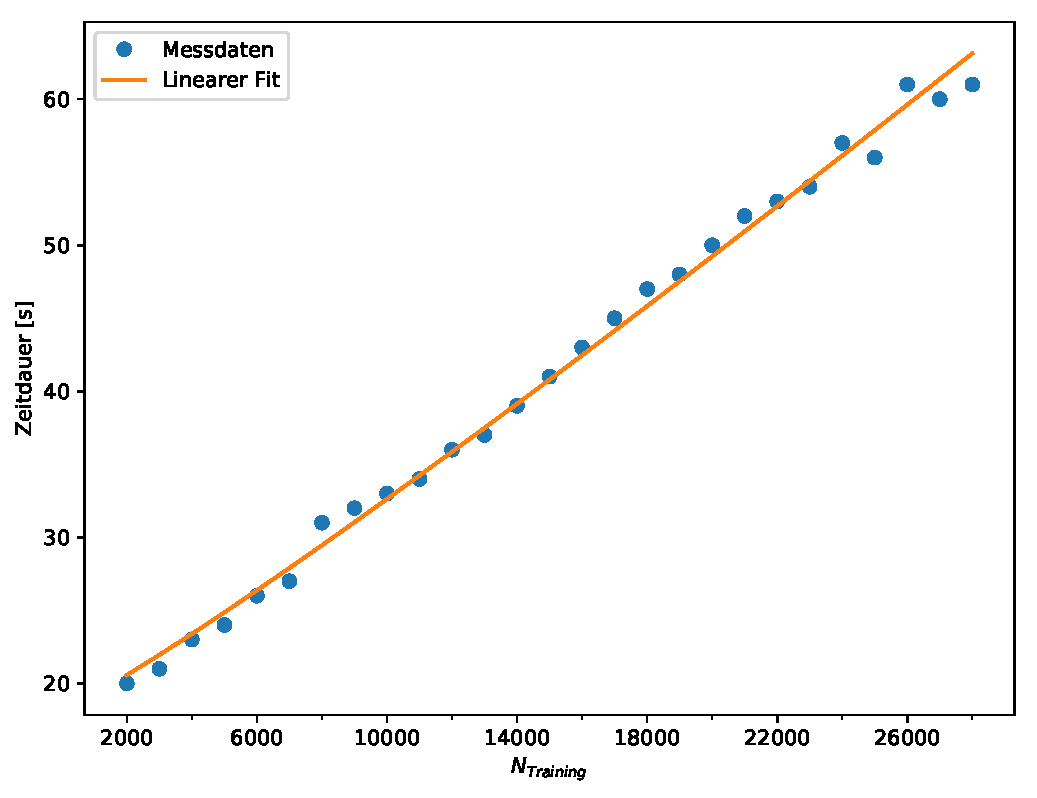
\includegraphics[width=.76\textwidth]{figures/results/cross_prediction/nn_trainlength_uv_time.pdf}
		\caption{Abhängigkeit der Laufzeit von $N_{Training}$.}
	\end{subfigure}%
	\\
	\begin{subfigure}{.95\textwidth}
		\centering
		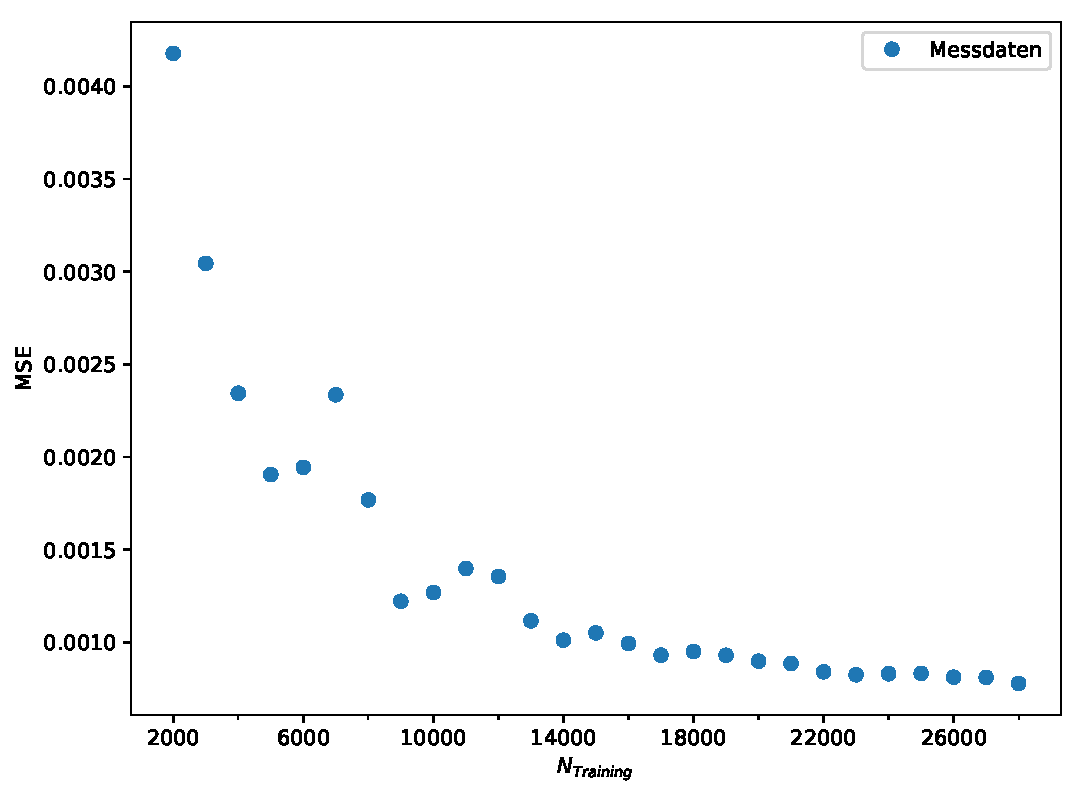
\includegraphics[width=.80\textwidth]{figures/results/cross_prediction/nn_trainlength_uv_mse.pdf}
		\caption{Abhängigkeit des \textit{MSE}s von $N_{Training}$.}
	\end{subfigure}%
	\caption{Darstellung der Abhängigkeit des benötigten Laufzeit (oben) und des MSE (unten) von der verwendeten Anzahl an Trainingsdaten $N_{Training}$ (unten) für das \textit{Barkley}-Modell bei der Verwendung einer nächsten Nachbar Vorhersage.}
	\label{fig:exp_cross_nn_trainlength_mse_time_barkley}
\end{figure}

Eine Analoge Darstellung für das \textit{Mitchell-Schaeffer}-Modell ist in \ref{fig:apx_exp_cross_nn_trainlength_mse_time_ms} zu finden. Anzumerken ist, dass die Sättigung des Fehlers im \textit{Barkley}-Modell schon ab etwa $N_{Training}=15000$ eintritt, doch beim \textit{Mitchell-Schaeffer}-Modell erst deutlich später. Dies ist ein Hinweis darauf, dass die Dynamiken im letzteren chaotischer und unregelmäßiger als bei ersten ablaufen. Zusammenfassend lässt sich somit die Wahl der Trainingslänge von $N_{Training} = 15000$ für alle Szenarien und alle drei Methoden damit begründen, dass man für die Nächste Nachbar Vorhersage, welche am empfindlichsten auf diese Länge reagiert, eine akzeptablen Kompromiss zwischen der Rechenzeit und der Genauigkeit erhält.

\FloatBarrier
\subsection{Radiale Basisfunktionen}
Bei der Verwendung radialer Basisfunktionen stellt zudem die Breite $\sigma_{RBF}$ der Gaußfunktionen als auch die Anzahl der Basisfunktionen $l$ einen wichtigen Parameter dar. Im Rahmen dieser Arbeit ist die Anzahl der Basisfunktionen auf $l=100$ festgelegt worden - diese Wahl wird im Folgenden weiter motiviert werden. Um die anderen Parameter zu finden, sind $\sigma$, $\Delta \sigma$ wie oben beschrieben, $\delta \in \{3,4,5\}$ und $\sigma_{RBF} \in \{0.5, 1.0, 3.0, 5.0, 7.0, 9.0\}$ variiert worden. In Tabelle \ref{tab:exp_cross_rbf_results} sind die dadurch gefundenen optimalen Parameter, die damit erreichten Fehler und die benötigte Laufzeit erneut für beide Modelle aufgelistet. Hierbei ist zu bemerken, dass die optimalen Werte für $\sigma$, $\Delta \sigma$ und $\delta$ mit denen für die NN-Vorhersage übereinstimmen. 

\begin{table}[h]
	\centering

	\begin{tabular}{ccc}
		\hline 			
		\multicolumn{1}{c}{} & Barkley & Mitchell-Schaeffer \\ 
		\hline 
		\rule[-1ex]{0pt}{2.5ex} $\sigma$ & $1$ & $7$ \\ 
		\rule[-1ex]{0pt}{2.5ex} $\Delta \sigma$ & $1$ & $1$ \\ 
		\rule[-1ex]{0pt}{2.5ex} $\delta$ & $3$ & $3$ \\ 
		\rule[-1ex]{0pt}{2.5ex} $\sigma_{RBF}$ & $0.5$ & $5$ \\ 
		\rule[-1ex]{0pt}{2.5ex} Laufzeit [s] & $1430$ & $1434$ \\ 
		\rule[-1ex]{0pt}{2.5ex} \textbf{MSE} & \textbf{0.01046} & \textbf{0.00948} \\ 
		\rule[-1ex]{0pt}{2.5ex} \textbf{NRMSE} & \textbf{0.1023} & \textbf{0.6228} \\ 
		\hline 
	\end{tabular} 
	\caption{Ermittelte Hyperparameter der radialen Basisfunktionen für das \textit{Mitchell-Schaeffer}- und das \textit{Barkley}-Modell, welche zu den geringsten Fehlern führen.}
	\label{tab:exp_cross_rbf_results}
\end{table} 

Analog zu der Untersuchung des Einflusses der Trainingslänge $N_{Training}$ bietet es sich für die radialen Basisfunktionen an, den Einfluss der Anzahl der verwendeten Basisfunktionen $l$ auf die Genauigkeit und die benötigte Laufzeit zu untersuchen, um die zuvor angegebene Wahl $l=100$ zu begründen. Dabei werden jeweils wieder die besten zuvor ermittelten Hyperparameter verwendet. Hierfür sind die gemessenen Laufzeiten gegen die Anzahl der Basisfunktionen $l$ in Abbildung \ref{fig:exp_cross_rbf_placements_time_barkley} für das \textit{Barkley}-Modell aufgetragen worden. Zusätzlich ist auch der Zusammenhang zwischen dem erreichten MSE und der Anzahl der Basisfunktionen in Abbildung \ref{fig:exp_cross_rbf_placements_mse_barkley} aufgetragen. Eine dazu analoge Darstellung für das \textit{Mitchell-Schaeffer}-Modell ist in Abbildung \ref{fig:apx_exp_cross_rbf_placements_time_mse_ms} zu finden. Es ist erneut anzunehmen, dass näherungsweise ein linearer Zusammenhang zwischen der Laufzeit und der Anzahl der Basisfunktionen auf dem untersuchten Bereich besteht.

\begin{figure}[h]
	\centering
	\begin{subfigure}{\textwidth}
		\centering
		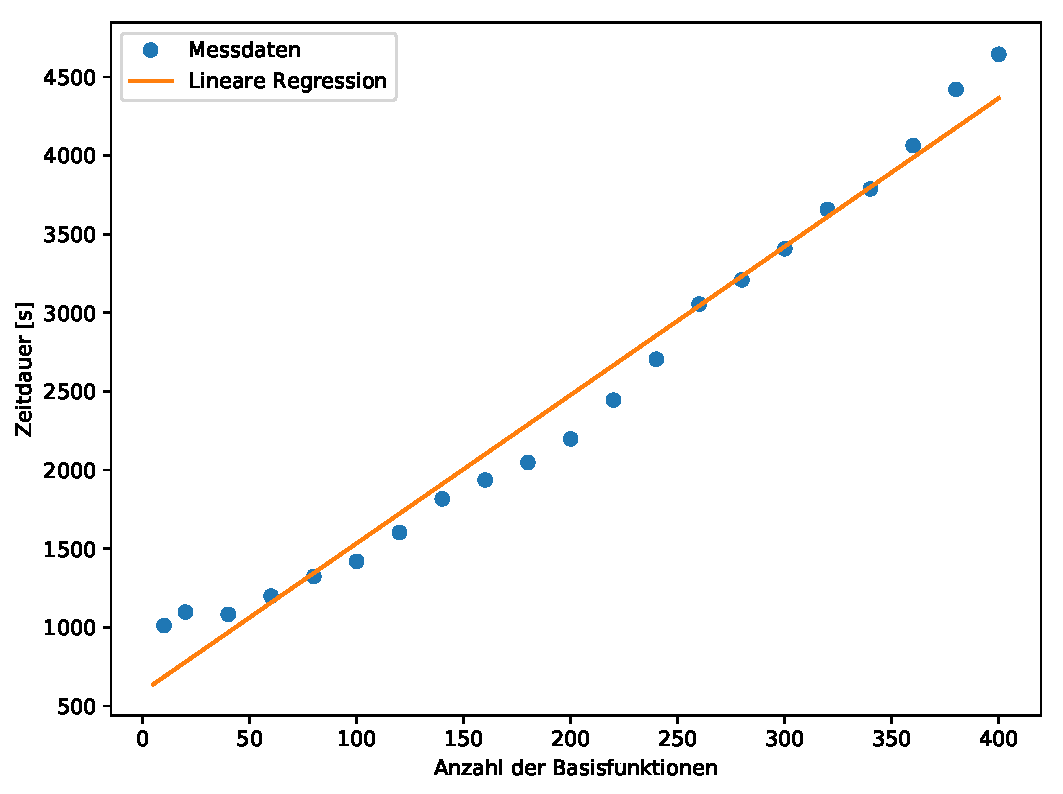
\includegraphics[width=4.2in]{figures/results/cross_prediction/rbf_placements_uv_time.pdf}
		\caption{Abhängigkeit der Laufzeit von $l$.}
	\end{subfigure}%
	\caption{Darstellung der Abhängigkeit des benötigten Laufzeit von der Anzahl der Basisfunktionen $l$ für das \textit{Barkley}-Modell\textit{Mitchell-Schaeffer}-Modell bei der Verwendung radialer Basisfunktionen.}
	\label{fig:exp_cross_rbf_placements_time_barkley}
\end{figure}

\begin{figure}[h]
	\centering
	\begin{subfigure}{\textwidth}
		\centering
		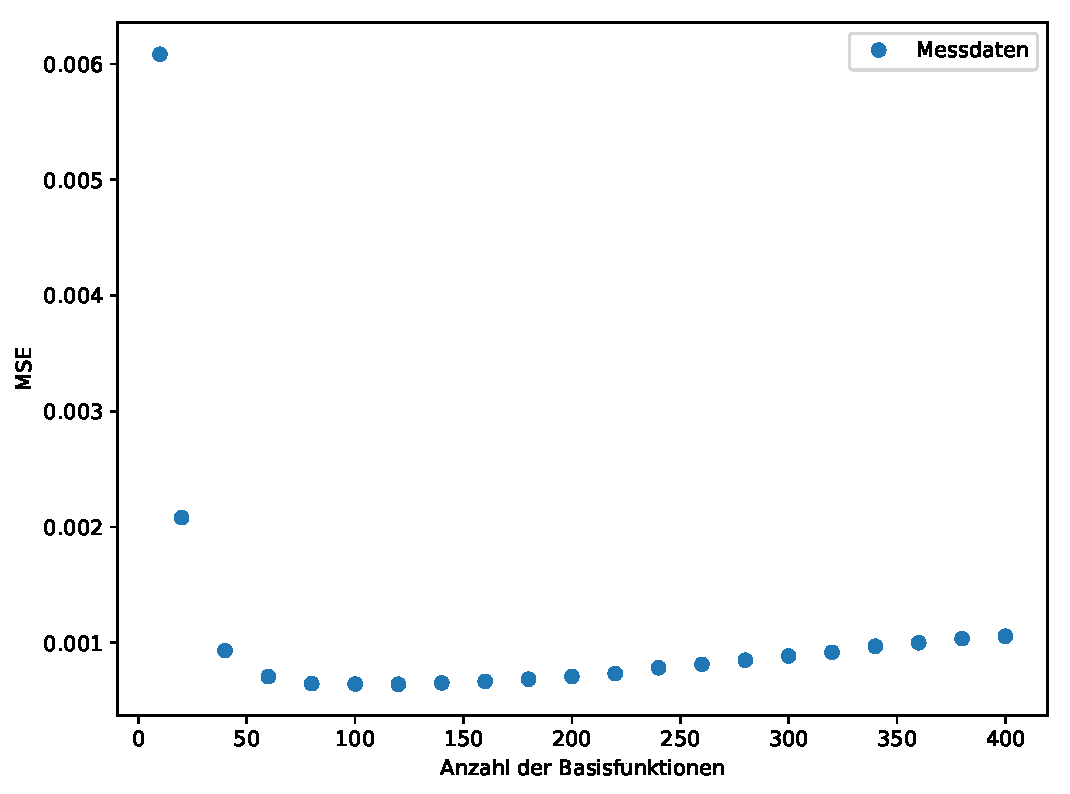
\includegraphics[width=4.2in]{figures/results/cross_prediction/rbf_placements_uv_mse.pdf}
  		\caption{Abhängigkeit des \textit{MSE}s von $l$.}
	\end{subfigure}%
	
	\caption{Darstellung der Abhängigkeit des MSE (unten) von der Anzahl der Basisfunktionen $l$ für das \textit{Barkley}-Modell\textit{Mitchell-Schaeffer}-Modell bei der Verwendung radialer Basisfunktionen.}
	\label{fig:exp_cross_rbf_placements_mse_barkley}
\end{figure}

Bei der Untersuchung des Zusammenhangs zwischen MSE und der Anzahl der Basisfunktionen kann zum einen ein asymptotischer Anteil erkannt werden, sodass der Fehler zuerst für mehr Basisfunktionen abnimmt. Allerdings lässt das Verhalten für das \textit{Mitchell-Schaeffer}-Modell erahnen, dass es hierbei einen optimalen Wert gibt, ab dem der Fehler wieder ansteigt. Dies kann durch eine schlechtere Generalisierung der Dynamik und ein zu starkes Anpassen und die Trainingsphase (auch bekannt als \textit{Overfitting}) erklärt werden. Zusammenfassend zeigt sich, dass die Wahl von $100$ Basisfunktionen eine akzeptable Abschätzung ist, sodass der Fehler möglichst gering ist und die Laufzeit auch gering gehalten wird. Diese Annahme wird im Folgenden ohne weitere qualitative Untersuchungen auf die anderen beiden Probleme übertragen, um den benötigten Rechenaufwand für die Parametersuche in einem angebrachten Rahmen zu halten.  

\FloatBarrier
\subsection{Echo State Network}
Abschließend ist dieses Problem nun mit den \textit{ESN}s gelöst worden. Dazu sind die Hyperparameter nach Abschnitt \ref{sec:exp_general_esn} gesucht worden. Die gefundenen Parameter und die damit erreichten Ergebnisse sind in Tabelle \ref{tab:exp_cross_esn_results} aufgelistet. Es ist auffällig, dass die optimalen Werte für $\sigma$ und $\Delta \sigma$ hier von denen der NN- und der RBF-Vorhersage abweichen. Auffällig ist, dass für beide Modelle die gleichen Hyperparameter die höchste Genauigkeit erzielen.\improvement{Add more details?} \\

\begin{table}[h]
	\centering
	\captionsetup{width=0.9\linewidth}
	\begin{tabular}{ccc}
		\hline		
		\multicolumn{1}{c}{} &  Barkley & Mitchell-Schaeffer \\ 
		\hline 
		\rule[-1ex]{0pt}{2.5ex} $\sigma$ & $3$ & $3$ \\ 
		\rule[-1ex]{0pt}{2.5ex} $\Delta \sigma$ & $1$ & $1$ \\ 
		\rule[-1ex]{0pt}{3.5ex} $N$ & $400$ & $400$ \\ 
		\rule[-1ex]{0pt}{3.5ex} $\rho(|\mathbf{W}|)$ & $0.95$ & $0.95$\\ 
		\rule[-1ex]{0pt}{3.5ex} $\alpha$ & $0.05$ & $0.05$ \\ 
		\rule[-1ex]{0pt}{3.5ex} $\epsilon$ & $0.1$ & $0.1$ \\ 
		\rule[-1ex]{0pt}{3.5ex} $\nu_{max}$ & $\num{1e-4}$ & $\num{1e-4}$\\ 
		\rule[-1ex]{0pt}{3.5ex} $\lambda$ & $\num{5e-6}$ & $\num{5e-6}$\\ 
		\rule[-1ex]{0pt}{2.5ex} Laufzeit [s] & $3710$ & $3733$ \\ 
		\rule[-1ex]{0pt}{2.5ex} \textbf{MSE} & \textbf{$\num{8.7e-7}$} & \textbf{0.00075} \\ 
		\rule[-1ex]{0pt}{2.5ex} \textbf{NRMSE} & \textbf{0.0039} & \textbf{0.1859} \\ 
		\hline 
	\end{tabular} 
	\caption{Ermittelte Hyperparameter des \textsc{ESN} für das \textit{Mitchell-Schaeffer}- und das \textit{Barkley}-Modell, welche zu den geringsten Fehlern führen.}
	\label{tab:exp_cross_esn_results}
\end{table}

Zuvor ist die Annahme getroffen worden, dass die Dynamik sich an jedem Punkt im Inneren des Feldes lokal ähnelt. Um diese Annahme zu untersuchen bietet es sich an die unterschiedlichen trainierten Gewichtsmatrizen $\mathbf{W_{out}}$ zu betrachten. Dies ist exemplarisch für die ermittelten Hyperparameter für das \textit{Barkley}-Modell durchgeführt und in Abbildung \ref{fig:exp_cross_esn_weights} dargestellt. Dabei gibt die vertikale Achse den Index $i$ des $i$-ten Eintrages von $\mathbf{W_{out}}$ an. Dafür sind die Matrizen $\mathbf{W_{out}} \in \mathbb{R}^{(1 + N_u + N) \times 1}$ mit $N_u = 9$ jeweils spaltenweise für $900$ Pixel in einem $30 \times 30$ Einheiten messendem Quadrat in der Mitte des Feldes aufgetragen.

\begin{figure}[H]
	\centering
	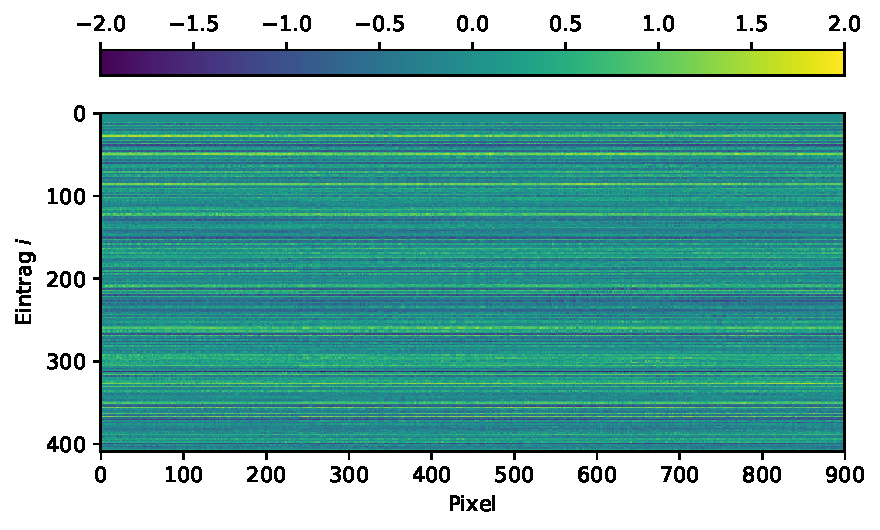
\includegraphics[height=3.0in]{figures/results/cross_prediction/weights.pdf}
	\setcapmargin[1cm]{1cm}
	\caption{Exemplarische Darstellung der Einträge der Gewichtsmatrix $\mathbf{W_{out}}$ des \textsc{ESN} für das \textit{Barkey}-Model anhand von $900$ verschiedene Bildpunkten, wobei$\mathbf{W_{out}}$ jeweils als Spalte in der Grafik dargestellt ist.}
	\label{fig:exp_cross_esn_weights}
\end{figure}

Dabei ist eine große Ähnlichkeit innerhalb der einzelnen Matrizen zu erkennen. So sind einige markante Linien in der Abbildung zu erkennen. So sind gewisse Einträge bei den Matrizen aller Pixel relativ stark beziehungsweise schwach. Trotzdem ist noch eine gewisse Varianz zuerkennen. Vermutlich wird sie dadurch verursacht, dass innerhalb der endlichen Trainingszeit nicht alle Dynamiken an jedem Pixel auftreten. Zusammenfassend kann dies als eine Bestätigung der Annahme der lokalen Ähnlichkeit gesehen werden. In weiteren Arbeiten bietet es sich an diese Frage weiter zu untersuchen und den Effekt dahingehend auszunutzen, als dass die Trainingsdaten mehrerer Punkte zusammengefasst werden können, sodass bereits aus einer kurzen Trainingszeit eine ausreichende Menge an Trainingsdaten gewonnen werden kann.
\improvement{Write something about the vanishing first 9 entries?}

\FloatBarrier
\subsection{Vergleich}
Abschließend kann nun ein Vergleich der drei verwendeten Methoden hinsichtlich ihrer Laufzeit und der erzielten Genauigkeiten durchgeführt werden. Dieser ist in Tabelle \ref{tab:exp_cross_comparison_results} zu finden. Die jeweils  besten Ergebnisse sind hervorgehoben. Die \textit{ESN}s erzielen für beide Modelle den geringsten Fehler, also die höchste Genauigkeit. Dabei ist der NRMSE für das \textit{Barkley}-Modell mehrere Größenordnung kleiner als bei den Konkurrenz-Ansätzen. Diese überaus hohe Genauigkeit ist für das \textit{Mitchell-Schaeffer}-Modell nicht erreicht worden. Hier beträgt der Fehler trotzdem etwa nur ein Drittel von dem der anderen Ansätze. Im Austausch für diese hohe Genauigkeit ist allerdings die benötigte Zeit für die Vorhersage höher als bei den Konkurrenten. Unter der Voraussetzung, dass die Rechenzeit nur eine untergeordnete Rolle spielt, so ergeben sich die \textit{ESN}s als bester Ansätze für die Kreuz-Prädiktion.
\begin{table}[h]
	\centering
	\captionsetup{width=0.9\linewidth}
	\begin{tabular}{cccccccc}
		\hline		
		\multicolumn{1}{c}{} & \multicolumn{3}{c}{Barkley} & \multicolumn{3}{c}{Mitchell-Schaeffer}		\\
		%\cline{2-7}
		\multicolumn{1}{c}{} & NN & RBF & ESN & NN & RBF & ESN \\
		
		\hline
		
		Laufzeit [s] 	& \textbf{40} 		& 1430		& 3710		& 5252		& \textbf{1434} 		& 3733 \\
		MSE 			& 0.00098	& 0.01046	& \textbf{\num{8.7e-7}} 	& 0.01891	& 0.00948 	& \textbf{0.00075} \\
		NRMSE 			& 0.1317	& 0.1023	& \textbf{\num{0.0039}} 	& 0.8795	& 0.6228 	& \textbf{0.1859} \\
		\hline 
	\end{tabular} 
	\caption{Vergleich der benötigten Laufzeit und der erreichten Fehlers der drei Ansätze für das \textit{Mitchell-Schaeffer}- und das \textit{Barkley}-Modell, welche zu den geringsten Fehlern führen.}
	\label{tab:exp_cross_comparison_results}
\end{table}

\FloatBarrier
\section{Prädiktion der Dynamik durch das Fernfeld}
\label{sec:exp_unblur}
Bei der Durchführung von invitro Experimenten mit Herzen gibt es verschiedene Möglichkeiten die Messung der elektrischen Erregung auf der Herzoberfläche durchzuführen. Zum einen können Elektroden zur Messung benutzt werden, zum anderen allerdings auch Fluoreszenzmessungen durchgeführt werden. Bei der Verwendung von Elektroden wird effektiv nicht das unmittelbare elektrische Feld auf der Herzoberfläche gemessen, sondern ein Fernfeld dessen. Es stellt sich nun die Frage, ob aus der Kenntnis dieses Fernfeldes die korrekte Erregung auf der Oberfläche bestimmt werden kann. Eine experimentelle Untersuchung dieser Fragestellung wird im Folgenden durchgeführt. Hierfür müssen zuerst diese Fernfeldaufnahmen für das \textit{Barkley}- und für das \textit{Mitchell-Schaeffer}-Modell erzeugt werden. Dabei wird das Fernfeld nicht korrekt simuliert, sondern durch eine gaußsche Unschärfe emuliert. Dazu wird auf das gesamte Feld der Spannungsvariable beider Modelle eine solche Unschärfe mit einer Breite $\sigma_{Blur} = 8.0$ mittels einer Faltung angewendet. Eine exemplarische Darstellung des emulierten Fernfeldes und des tatsächlichen Feldes ist in Abbildungen \ref{fig:exp_unblur_barkley} und \ref{fig:exp_unblur_mitchell_schaeffer} zu finden.

\begin{figure}[h]
	\centering
	\begin{subfigure}{.5\textwidth}
		\centering
		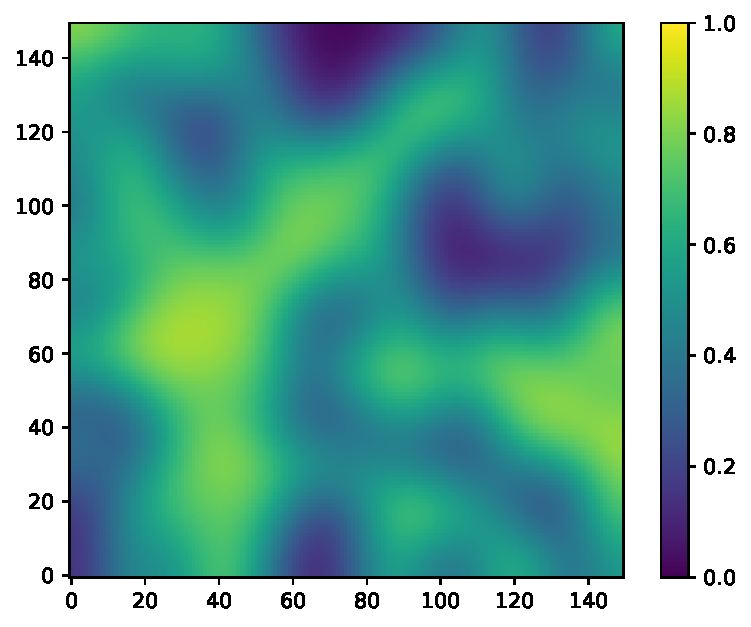
\includegraphics[height=2.5in]{figures/results/unblur/barkley_u_blur_blured.pdf}
		\setcapmargin[1cm]{1cm}
		\caption{Emuliertes Fernfeld}
		\label{fig:exp_unblur_barkley_blurred}
	\end{subfigure}%
	\begin{subfigure}{.5\textwidth}
		\centering
		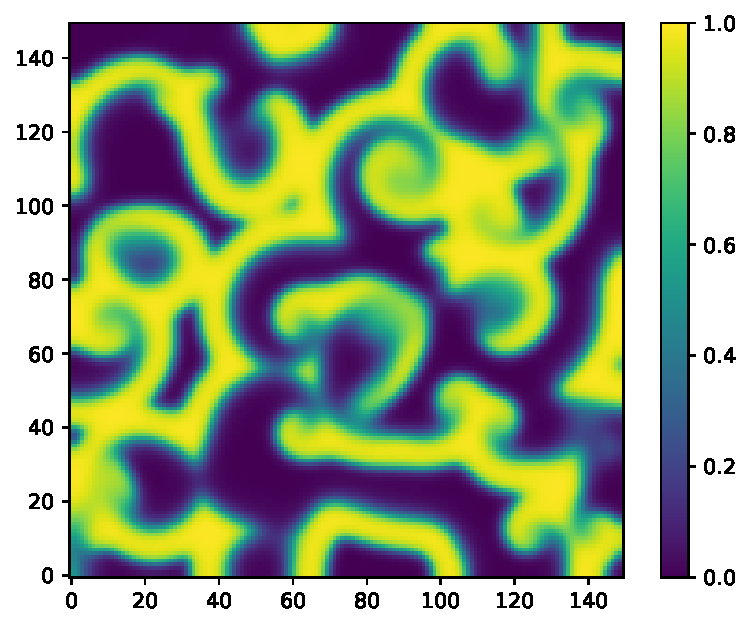
\includegraphics[height=2.5in]{figures/results/unblur/barkley_u_blur_orig.pdf}
		\setcapmargin[1cm]{1cm}
  		\caption{Echte Erregung des Modells}
  		\label{fig:exp_unblur_barkley_orig}
	\end{subfigure}
	\caption{Graphische Darstellung der $u$-Variable des \textit{Barkley}-Modells. Links ist das emulierte Fernfeld und rechts das tatsächliche $u$-Feld des Modells zu sehen.}
	\label{fig:exp_unblur_barkley}
\end{figure} 

\begin{figure}[h]
	\centering
	\begin{subfigure}{.5\textwidth}
		\centering
		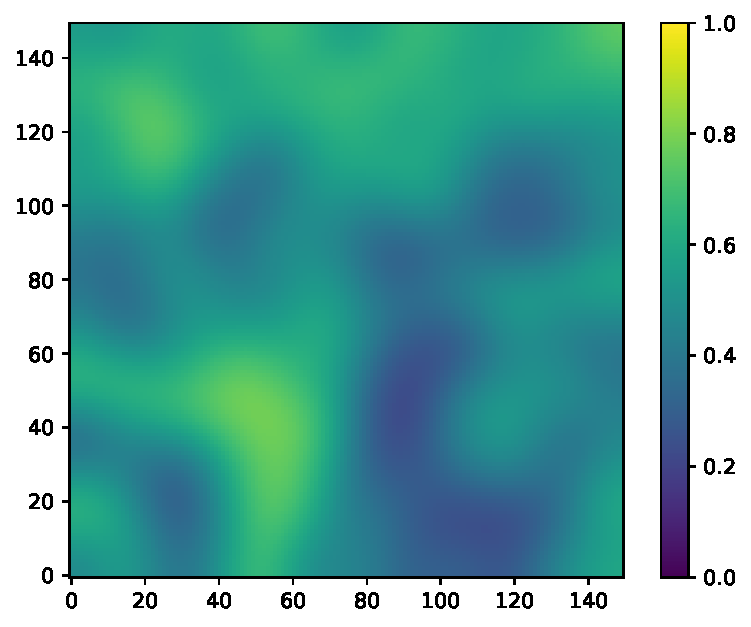
\includegraphics[height=2.5in]{figures/results/unblur/mitchell_v_blur_blured.pdf}
		\setcapmargin[1cm]{1cm}
		\caption{Emuliertes Fernfeld}
		\label{fig:exp_unblur_mitchell_schaeffer_blurred}
	\end{subfigure}%
	\begin{subfigure}{.5\textwidth}
		\centering
		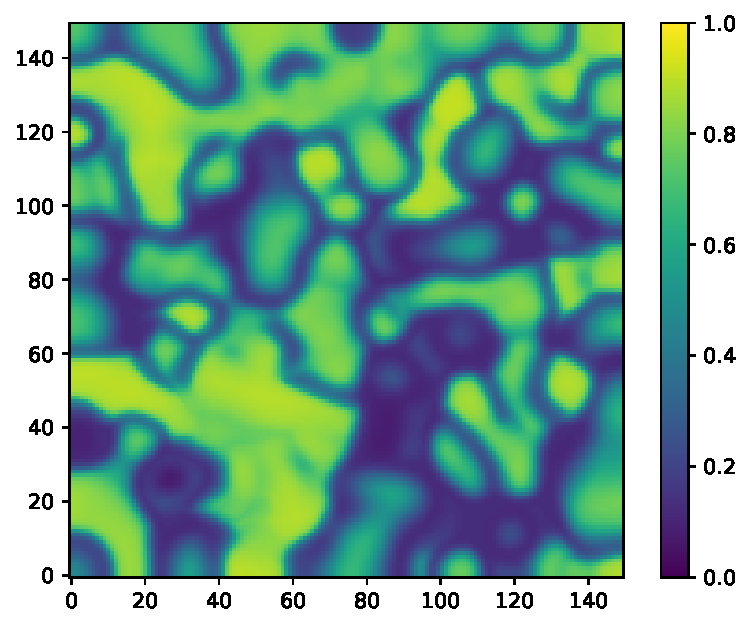
\includegraphics[height=2.5in]{figures/results/unblur/mitchell_v_blur_orig.pdf}
		\setcapmargin[1cm]{1cm}
  		\caption{Echte Erregung des Modells}
  		\label{fig:exp_unblur_mitchell_schaeffer_orig}
	\end{subfigure}
	\caption{Graphische Darstellung der $v$-Variable des \textit{Mitchell-Schaeffer}-Modells. Links ist das emulierte Fernfeld und rechts das tatsächliche $v$-Feld des Modells zu sehen.}
	\label{fig:exp_unblur_mitchell_schaeffer}
\end{figure} 

\subsection{Nächste Nachbar Vorhersage}
Zuerst wird diese Aufgabe erneut mit dem \textsc{NN}-Ansatz betrachtet. Die besten gefundenen Hyperparameter dafür sind in Tabelle \ref{tab:exp_unblur_nn_results} aufgelistet. Bemerkenswert ist erneut die geringe Laufzeit dieses Ansatzes. Dies wird durch die verhältnismäßig geringe Dimensionalität des Eingabe-Vektors begünstigt. Allerdings sind die Fehlerwerte sehr hoch, sodass die Vorhersage kaum besser ist, als eine Schätzung mit dem Mittelwert als Vorhersage.

\begin{table}[h]
	\centering

	\begin{tabular}{|c|c|c|}
		\multicolumn{1}{c|}{} & Barkley & Mitchell-Schaeffer \\ 
		\hline \hline 
		\rule[-1ex]{0pt}{2.5ex} $\sigma$ & $1$ & $1$ \\ 
		\hline 
		\rule[-1ex]{0pt}{2.5ex} $\Delta \sigma$ & $1$ & $1$ \\ 
		\hline 
		\rule[-1ex]{0pt}{2.5ex} $\delta$ & $4$ & $3$ \\ 
		\hline 
		\rule[-1ex]{0pt}{2.5ex} k & $5$ & $5$ \\ 
		\hline 
		\rule[-1ex]{0pt}{2.5ex} Laufzeit [s] & $53$ & $42$ \\ 
		\hline 
		\rule[-1ex]{0pt}{2.5ex} \textbf{MSE} & \textbf{0.10089} & \textbf{0.06217} \\ 
		\hline 
		\rule[-1ex]{0pt}{2.5ex} \textbf{NRMSE} & \textbf{0.8227} & \textbf{0.9136} \\ 
		\hline 
	\end{tabular} 

	\caption{Gefundene Hyperparameter der nächsten Nachbar Vorhersage für das \textit{Mitchell-Schaeffer}- und das \textit{Barkley}-Modell, welche zu den geringsten Fehlern führen.}
\label{tab:exp_unblur_nn_results}
\end{table} 


\FloatBarrier
\subsection{Radiale Basisfunktionen}
Als nächstes sind nun die radialen Basisfunktionen ebenfalls auf das Problem angewendet worden. Die dabei gefundenen Hyperparameter sind in Tabelle \ref{tab:exp_unblur_rbf_results} präsentiert.

\begin{table}[h]
	\centering

	\begin{tabular}{|c|c|c|}
		\multicolumn{1}{c|}{} & Barkley & Mitchell-Schaeffer \\ 
		\hline \hline 
		\rule[-1ex]{0pt}{2.5ex} $\sigma$ & $3$ & $5$ \\ 
		\hline 
		\rule[-1ex]{0pt}{2.5ex} $\Delta \sigma$ & $1$ & $2$ \\ 
		\hline 
		\rule[-1ex]{0pt}{2.5ex} $\delta$ & $3$ & $3$ \\ 
		\hline 
		\rule[-1ex]{0pt}{2.5ex} $\sigma_{RBF}$ & $5.0$ & $9.0$ \\ 
		\hline 
		\rule[-1ex]{0pt}{2.5ex} Laufzeit [s] & $1840$ & $1842$ \\ 
		\hline 
		\rule[-1ex]{0pt}{2.5ex} \textbf{MSE} & \textbf{0.03899} & \textbf{0.03252} \\ 
		\hline 
		\rule[-1ex]{0pt}{2.5ex} \textbf{NRMSE} & \textbf{0.5114} & \textbf{0.6913} \\ 
		\hline 
	\end{tabular} 
	\caption{Gefundene Hyperparameter der radialen Basisfunktionen für das \textit{Mitchell-Schaeffer}- und das \textit{Barkley}-Modell, welche zu den geringsten Fehlern führen.}
	\label{tab:exp_unblur_rbf_results}
\end{table} 


\FloatBarrier
\subsection{Echo State Network}
Nachdem die klassischen Methoden bereits auf dieses Problem angewendet worden sind, kann das Problem nun mittels der \textsc{ESN}s erneut betrachtet werden. Hierfür sind die verwendeten Hyperparameter erneut nach Abschnitt \ref{sec:exp_general_esn} gesucht worden. Die Ergebnisse sind in Tabelle \ref{tab:exp_unblur_esn_results} zu finden. Auffällig ist hierbei, dass die optimale Größe $N$ des Reservoirs für beiden Modelle unter der maximal betrachteten Größe $N \leq 400$ liegt. Dies kann ein Anzeichen dafür sein, dass für das Bewältigen der Aufgabe kein ausgeprägtes Langzeitgedächtnis vorhanden sein muss, da diese nach Abschnitt \ref{sc:esn} mit der Größe $N$ des Reservoirs skaliert. 
\improvement{Add more details on:long time memory vs N dependency in theory.}

\begin{table}[h]
	\centering
	\captionsetup{width=0.9\linewidth}
	\begin{tabular}{|c|c|c|}
		\multicolumn{1}{c|}{} &  Barkley & Mitchell-Schaeffer \\ 
		\hline \hline 
		\rule[-1ex]{0pt}{2.5ex} $\sigma$ & $7$ & $7$ \\ 
		\hline 
		\rule[-1ex]{0pt}{2.5ex} $\Delta \sigma$ & $1$ & $1$ \\ 
		\hline 
		\rule[-1ex]{0pt}{3.5ex} $N$ & $200$ & $50$ \\ 
		\hline 
		\rule[-1ex]{0pt}{3.5ex} $\rho(|\mathbf{W}|)$ & $1.50$ & $0.10$\\ 
		\hline 
		\rule[-1ex]{0pt}{3.5ex} $\alpha$ & $0.20$ & $0.05$ \\ 
		\hline 
		\rule[-1ex]{0pt}{3.5ex} $\epsilon$ & $0.1$ & $0.1$ \\ 
		\hline 
		\rule[-1ex]{0pt}{3.5ex} $\nu_{max}$ & $\num{1e-5}$ & $\num{1e-4}$\\ 
		\hline 
		\rule[-1ex]{0pt}{3.5ex} $\lambda$ & $\num{5e-10}$ & $\num{5e-6}$\\ 
		\hline 
		\rule[-1ex]{0pt}{2.5ex} Laufzeit [s] & $1603$ & $1540$ \\ 
		\hline 
		\rule[-1ex]{0pt}{2.5ex} \textbf{MSE} & \textbf{0.02347} & \textbf{0.02449} \\ 
		\hline
		\rule[-1ex]{0pt}{2.5ex} \textbf{NRMSE} & \textbf{0.3968} & \textbf{0.3599} \\ 
		\hline 
	\end{tabular} 
	\caption{Gefundene Hyperparameter des \textsc{ESN} für das \textit{Mitchell-Schaeffer}- und das \textit{Barkley}-Modell, welche zu den geringsten Fehlern führen.}
	\label{tab:exp_unblur_esn_results}
\end{table}

\FloatBarrier
\subsection{Vergleich}
Zusammenfassend können nun die Ergebnisse der drei Ansätze erneut verglichen werden. Eine vergleichende Übersicht ist in Tabelle \ref{tab:exp_unblur_esn_results} zu finden. Dort ist erneut zu bemerken, dass die \textsc{ESN}s die geringsten Fehlerwerte erzeugt, doch der \textsc{NN}-Ansatz deutlich schneller berechnet werden kann.\\
Zusätzlich zu der Tabelle ist noch ein exemplarischer grafischer Vergleich der Resultate der drei Ansätze mit dem Ziel in Abbildung \ref{fig:exp_unblur_barkley_result} dargestellt. Dort fällt auf, dass die Vorhersage des \textsc{NN}-Ansatzes selbst die Struktur der Dynamik kaum korrekt auflöst. Im Vergleich dazu ist die Vorhersage des \textsc{RBF}-Ansatzes und des \textsc{ESN} deutlich feiner und beinhaltet sogar die Makrostruktur der Dynamik. Des Weiteren ist zu bemerken, dass diese mit dem \textsc{ESN} leicht feiner aufgelöst worden ist, als mit \textsc{RBF}-Ansatz. Zwar stimmen hier auch nicht die feinen Details der Dynamik mit dem Original überein, doch ist eine starke Verbesserung im Vergleich zu dem emulierten Fernfeld zu bemerken. Unter Umständen wäre es für zukünftige Arbeiten bei dieser Aufgabe angebracht eine andere Fehlermetrik als die mittlere quadratische Abweichung zu benutzen, welche die Ähnlichkeit zwischen den Strukturen der Felder stärker berücksichtigt. 

\begin{figure}[h]
	\centering
	\begin{subfigure}{.5\textwidth}
		\centering
		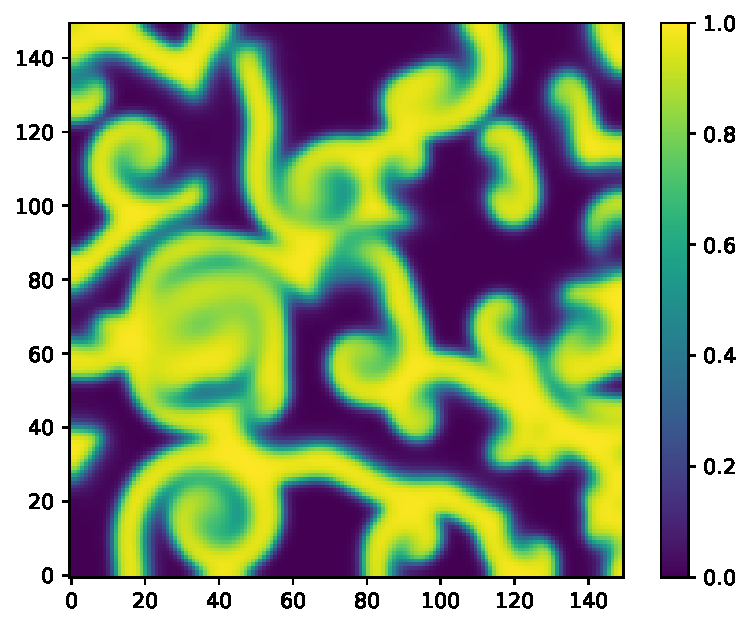
\includegraphics[height=2.5in]{figures/results/unblur/esn_barkley_u_blur_orig.pdf}
		\setcapmargin[1cm]{0.5cm}
		\caption{Echte Erregung des Modells}
		\label{fig:exp_unblur_barkley_result_orig}
	\end{subfigure}%
	\begin{subfigure}{.5\textwidth}
		\centering
		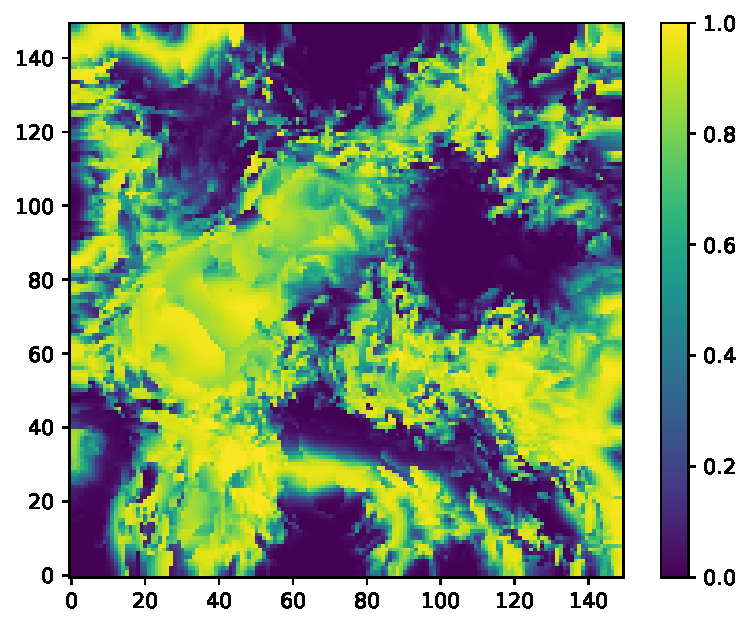
\includegraphics[height=2.5in]{figures/results/unblur/nn_barkley_u_blur_pred.pdf}
		\setcapmargin[1cm]{0.5cm}
  		\caption{Vorhersage des \textsc{NN}-Ansatzes}
  		\label{fig:exp_unblur_barkley_result_nn_pred}
	\end{subfigure}
	\begin{subfigure}{.5\textwidth}
		\centering
		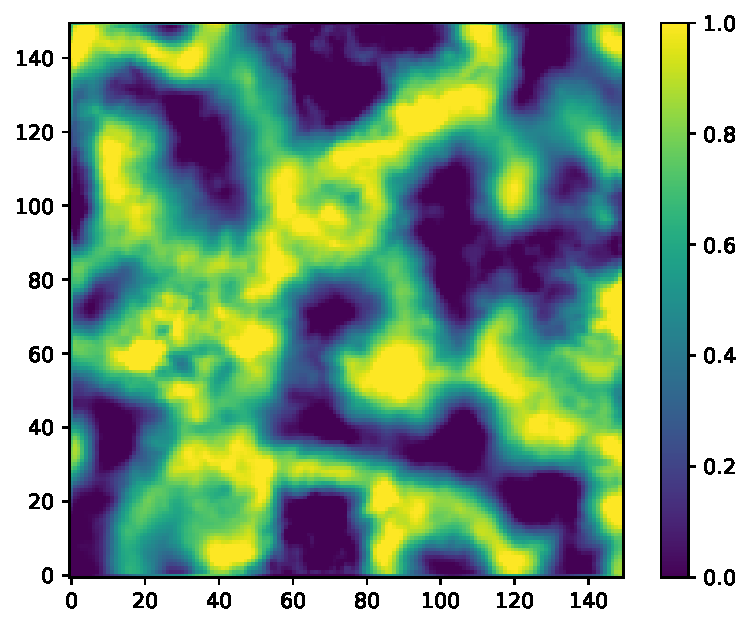
\includegraphics[height=2.5in]{figures/results/unblur/rbf_barkley_u_blur_pred.pdf}
		\setcapmargin[1cm]{0.5cm}
  		\caption{Vorhersage des \textsc{RBF}-Ansatzes}
  		\label{fig:exp_unblur_barkley_result_rbf_pred}
	\end{subfigure}%
	\begin{subfigure}{.5\textwidth}
		\centering
		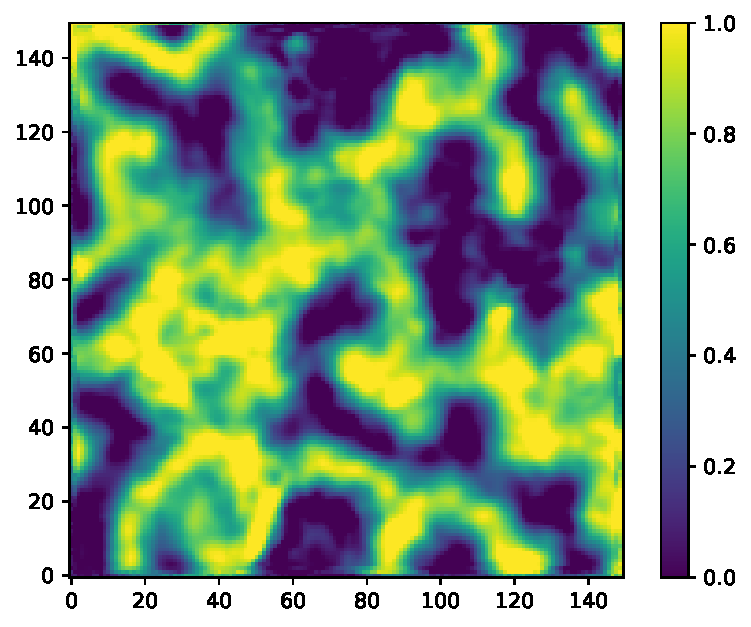
\includegraphics[height=2.5in]{figures/results/unblur/esn_barkley_u_blur_pred.pdf}
		\setcapmargin[1cm]{0.5cm}
  		\caption{Vorhersage des \textsc{ESN}}
  		\label{fig:exp_unblur_barkley_result_esn_pred}
	\end{subfigure}
	\caption{Graphische Darstellung der $u$-Variable des \textit{Barkley}-Modells für den $100$. Zeitschritt des Testdatensatzes. Oben links ist das tatsächliche Feld des Modells zu sehen. Danach folgenden im Uhrzeigersinn die Vorhersagen des \textsc{NN}-Ansatzes, des \textsc{RBF}-Ansatzes und des \textsc{ESN}.}
	\label{fig:exp_unblur_barkley_result}
\end{figure} 

\begin{table}[h]
	\centering
	\captionsetup{width=0.9\linewidth}
	\begin{tabular}{|c|c|c|c|c|c|c|c|}
		\multicolumn{1}{c|}{} & \multicolumn{3}{c|}{Barkley} & \multicolumn{3}{c|}{Mitchell-Schaeffer}		\\
		\cline{2-7}
		\multicolumn{1}{c|}{} & NN & RBF & ESN & NN & RBF & ESN \\
		
		\hline
		\hline
		
		Laufzeit [s] 	& \textbf{53} 	& 1840		& 3604				& \textbf{42}	& 1842 		& 3823 \\
		\hline
		MSE 			& 0.10089		& 0.03899	& \textbf{0.02347} 	& 0.06217		& 0.03252 	& \textbf{0.02449} \\
		\hline
		NRMSE 			& 0.8227		& 0.5114	& \textbf{0.3968} 	& 0.9136		& 0.6913 	& \textbf{0.3599} \\
		\hline 
	\end{tabular} 
	\caption{Vergleich der benötigten Laufzeit und der erreichten Fehlers der drei Ansätze für das \textit{Mitchell-Schaeffer}- und das \textit{Barkley}-Modell, welche zu den geringsten Fehlern führen.}
	\label{tab:exp_unblur_comparison_results}
\end{table}

\FloatBarrier
\section{Kreuz-Prädiktion innere Dynamiken}
\label{sec:exp_inner_prediction}
Bei Messungen der elektrischen Erregung des Herzens können nach aktuellen Stand meistens nur die Erregungen auf der Herzoberfläche gemessen werden. Die Ausbreitungen im Inneren des räumlich ausgedehnten Herzens bleiben somit verborgen. Zudem ist anzunehmen, dass die Gesamtdynamik nicht nur durch die Oberfläche, sondern auch durch die Erregung im Inneren bestimmt und charakterisiert wird. Somit wird die Frage aufgeworfen, ob die innere Erregung des Herzens nur durch die Kenntnis der Oberflächendynamik vorhergesagt werden kann. In diesem Abschnitt soll versucht werden, diese Fragestellung erneut mit den \textsc{ESN}s und den klassischen Methoden zu untersuchen. Dabei wird diese Frage statt an einem dreidimensionalen Systems an den zuvor bereits benutzten zweidimensionalen Modellen untersucht.\\

\begin{figure}[h]
	\centering
	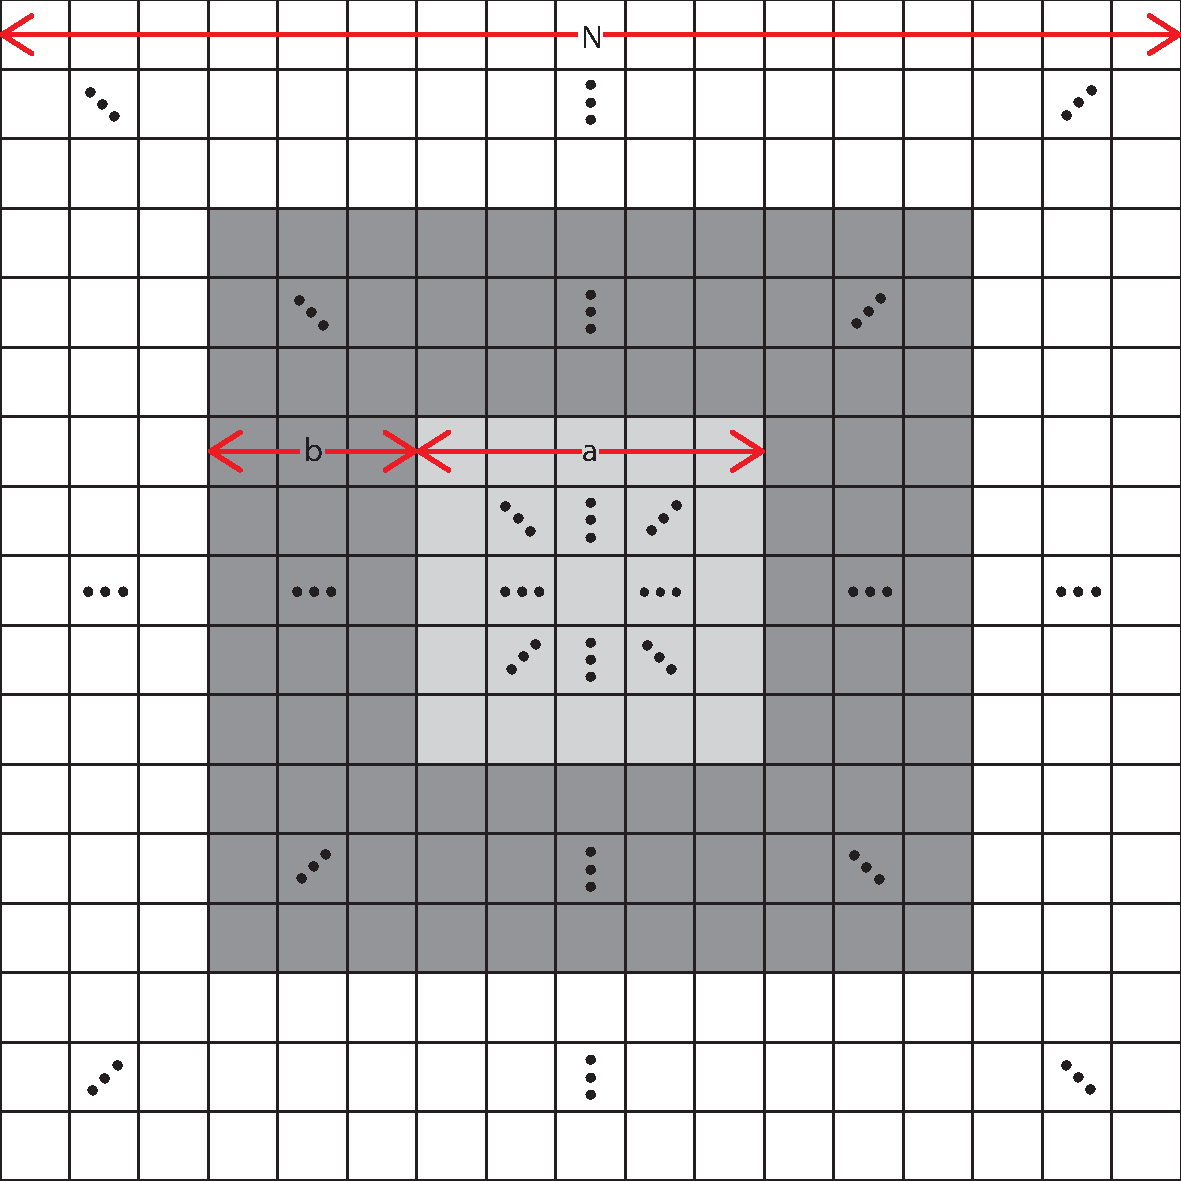
\includegraphics[width=.4\linewidth]{figures/illustrations/inner_prediction.pdf}
	\caption{Darstellung des Aufbaus. Das gesamte $N \times N$ große Feld der Spannungsvariable ist in weiß, wohingegen der vorherzusagende Bereich der Größe $a \times a$ in hellgrau dargestellt ist. Drumherum liegt der dunkelgraue Rahmen der Größe $b \times b$ dessen Pixel für die Vorhersage des Inneren genutzt werden.}
	\label{fig:exp_inner_prediction}
\end{figure}

Hierbei wird nur das Feld der Spannungsvariable betrachtet. In diesem $N \times N$ Einheiten großem Feld wird ein Quadrat mit der Seitenlänge $a$ ausgewählt, für dessen Pixel die Spannungsvariable bestimmt werden soll. Dazu wird um das innere Quadrat ein Rahmen der Breite $b$ gewählt und die Spannungsvariable der beinhalteten Pixel als Quelle genutzt. Eine graphische Illustration dieses Aufbaus ist in Abbildung \ref{fig:exp_inner_prediction} dargestellt. Somit wird die Spannung im Inneren für $a^2$ Punkte durch die Kenntnis der $(a+2b)^2-a^2$ umgebenden Pixel bestimmt.\\

Dieses Szenario ist für die in Tabelle \ref{tab:exp_inner_cross_pred_parameter} angegebenen Parameterkombinationen durchgeführt worden. Im Folgenden werden jeweils nur die gefundenen Hyperparameter und Ergebnisse für den $b$ Wert vorgestellt, der zu dem geringsten Fehler führt.

\begin{table}[h]
	\centering
	\begin{tabular}{cccc|ccc|ccc|ccc|ccc|ccc|cc|c}
		\hline
		$a$ & \multicolumn{3}{c|}{4} & \multicolumn{3}{c|}{8} & \multicolumn{3}{c|}{16} & \multicolumn{3}{c|}{32} & \multicolumn{3}{c|}{64} & \multicolumn{3}{c|}{128*} & \multicolumn{2}{c|}{146*} & 148* \\
		\hline
		$b$ & 1 & 2 & 3 & 1 & 2 & 3 & 1 & 2 & 3 & 1 & 2 & 3 & 1 & 2 & 3 & 1 & 2 & 3 & 2 & 1 & 1 \\
		\hline
	\end{tabular} 
	\caption{Verwendete Parameter $a$ und $b$ für die Abmessungen des inneren und äußeren Quadrates. Die markierten Werte sind nur für die \textsc{ESN}s untersucht worden.}
	\label{tab:exp_inner_cross_pred_parameter}
\end{table} 

\subsection{Nächste Nachbar Vorhersage}
Für die letzte Aufgabe ist erneut zuerst der \textsc{NN}-Ansatz getestet worden. Es ist anzumerken, dass dies nicht alle Parameterkombinationen $a$, $b$ aus Tabelle \ref{tab:exp_inner_cross_pred_parameter} durchgeführt worden ist, da der Rechenaufwand teilweise zu groß geworden ist. Dies liegt daran, dass die Dimension der Eingabevariablen mit
\begin{align*}
(a+2b)^2-a^2 = 4b^2+4ab
\end{align*}
skaliert. Da zudem die Rechenzeit für diesen Ansatz nach \ref{sc:theory_nn} für wachsende Dimensionen sehr stark zunimmt, kann diese Aufgabe für große Abmessungen des vorherzusagendenen Bereiches nicht mehr in einer angebrachten Zeit berechnet werden.
Die optimalen gefundenen Hyperparameter und die damit erreichten Ergebnisse sind in Tabelle \ref{tab:exp_inner_cross_nn_results} aufgelistet.

\begin{table}[h]
	\centering

	\begin{tabular}{ccccccccccc}
		\hline		
		\multicolumn{1}{c}{} & \multicolumn{5}{c}{Barkley}\\ 
		\hline 
		\rule[-1ex]{0pt}{2.5ex} $a$ & 4 & 8 & 16 & 32 & 64\\ 
		\rule[-1ex]{0pt}{2.5ex} $b$ & 1 & 1 & 1  & 1  & 1 \\ 
		\rule[-1ex]{0pt}{2.5ex} $\delta$ & 4 & 4 & 4 & 3 & 3 \\ 
		\rule[-1ex]{0pt}{2.5ex} k & 5 & 5 & 5 & 5 & 5 \\ 
		\rule[-1ex]{0pt}{2.5ex} Laufzeit [s] & $\approx 1$ & 8 & 287 & 1809 & 14754\\ 
		\rule[-1ex]{0pt}{2.5ex} \textbf{MSE} & \textbf{0.00231} & \textbf{0.00891} & \textbf{0.07097} & \textbf{0.18961} & \textbf{0.24599}\\ 
		\rule[-1ex]{0pt}{2.5ex} \textbf{NRMSE} & \textbf{0.0155} & \textbf{0.0596} & \textbf{0.4779} & \textbf{1.3032} & \textbf{1.7009} \\ 
		\hline 
	\end{tabular} 
	
	\vspace{0.75cm}

	\centering

	\begin{tabular}{ccccccccccc}
		\hline
		\multicolumn{1}{c}{} & \multicolumn{5}{c}{Mitchell-Schaeffer} \\ 
		\hline 
		\rule[-1ex]{0pt}{2.5ex} $a$ & 4 & 8 & 16 & 32 & 64 \\ 
		\rule[-1ex]{0pt}{2.5ex} $b$ & 1 & 1 & 1  & 1  & 1\\ 
		\rule[-1ex]{0pt}{2.5ex} $\delta$ & 3 & 3 & 3 & 4 & 4 \\ 
		\rule[-1ex]{0pt}{2.5ex} k & 5 & 5 & 5 & 5 & 5 \\ 
		\rule[-1ex]{0pt}{2.5ex} Laufzeit [s] & $\approx 1$ & 17 & 194 & 2482 & 20272\\ 
		\rule[-1ex]{0pt}{2.5ex} \textbf{MSE} & \textbf{0.14221} & \textbf{0.02465} & \textbf{0.06460} & \textbf{0.08744} & \textbf{0.09283} \\ 
		\rule[-1ex]{0pt}{2.5ex} \textbf{NRMSE} & \textbf{0.2663} & \textbf{0.4052} & \textbf{0.9779} & \textbf{1.3564} & \textbf{1.4012} \\ 
		\hline 
	\end{tabular} 

	\caption{Ermittelte Hyperparameter der nächsten Nachbar Vorhersage und Werte für $b$ für das \textit{Barkley}-Modell (oben) und das \textit{Mitschell-Schaeffer}-Modell (unten) für verschiedene Größen $a$ des vorherzusagenden Bereichs, welche zu den geringsten Fehlern führen.}
\label{tab:exp_inner_cross_nn_results}
\end{table}

Dabei ist zu erkennen, dass die Qualität der Vorhersage mit steigendem $a$ stark abnimmt. So kann für das \textit{Barkley}-Modell nur für $a \in \{4,8\}$ ein NRMSE der deutlich unter $0.50$ erreicht werden. Für größere Bereiche steigt der NRMSE sogar auf $> 1.0$ an, sodass die Vorhersage nicht mehr genauer ist als eine naive Vorhersage mittels des Mittelwertes des Trainingsdatensatzes. Die Vorhersagen des \textit{Mitchell-Schaeffer}-Modells zeigen eine gleichartige Tendenz, doch ist hier der Fehler für die kleinste innere Abmessung $a=4$ deutlich stärker als im \textit{Barkley}-Modell.

\FloatBarrier
\subsection{Radiale Basisfunktionen}
Analog zu den vorherigen Ausführungen sind die radialen Basisfunktionen ebenfalls auf dieses Problem angewendet worden. Dabei ist mit einer analogen Begründung wie bei den nächsten Nachbarn nur der eingeschränkte Wertebereich für $a$ durchlaufen worden. Die dafür gefundenen Hyperparameter und die Fehler können in Tabelle \ref{tab:exp_inner_cross_rbf_results} gefunden werden.
\begin{table}[h]
	\centering

	\begin{tabular}{ccccccccccc}
		\hline
		\multicolumn{1}{c}{} & \multicolumn{5}{c}{Barkley}\\ 
		\hline
		\rule[-1ex]{0pt}{2.5ex} $a$ & 4 & 8 & 16 & 32 & 64\\ 
		\rule[-1ex]{0pt}{2.5ex} $b$ & 1 & 1 & 1  & 1  & 1 \\ 
		\rule[-1ex]{0pt}{2.5ex} $\delta$ & 4 & 4 & 4 & 3 & 3 \\ 
		\rule[-1ex]{0pt}{2.5ex} $\sigma_{RBF}$ & 9 & 5 & 9 & 9 & 7\\ 
		\rule[-1ex]{0pt}{2.5ex} Laufzeit [s] & $\approx 2$ & 7 & 41 & 279 & 1845\\ 
		\rule[-1ex]{0pt}{2.5ex} \textbf{MSE} & \textbf{0.00051} & \textbf{0.00450} & \textbf{0.04009} & \textbf{0.08783} & \textbf{0.13615}\\ 
		\rule[-1ex]{0pt}{2.5ex} \textbf{NRMSE} & \textbf{0.0586} & \textbf{0.1735} & \textbf{0.5196} & \textbf{0.7769} & \textbf{0.9703} \\ 
		\hline 
	\end{tabular} 
	
	\vspace{0.75cm}

	\centering

	\begin{tabular}{ccccccccccc}
		\hline
		\multicolumn{1}{c}{} & \multicolumn{5}{c}{Mitchell-Schaeffer} \\ 
		\hline 
		\rule[-1ex]{0pt}{2.5ex} $a$ & 4 & 8 & 16 & 32 & 64 \\ 
		\rule[-1ex]{0pt}{2.5ex} $b$ & 1 & 1 & 1  & 1  & 1\\ 
		\rule[-1ex]{0pt}{2.5ex} $\delta$ & 3 & 3 & 3 & 4 & 4 \\ 
		\rule[-1ex]{0pt}{2.5ex} $\sigma_{RBF}$ & 9 & 9 & 9 & 5 & 7 \\ 
		\rule[-1ex]{0pt}{2.5ex} Laufzeit [s] & $\approx 1$ & 7 & 43 & 237 & 1756\\
		\rule[-1ex]{0pt}{2.5ex} \textbf{MSE} & \textbf{0.00064} & \textbf{0.00497} & \textbf{0.02220} & \textbf{0.04745} & \textbf{0.05588} \\ 
		\rule[-1ex]{0pt}{2.5ex} \textbf{NRMSE} & \textbf{0.1094} & \textbf{0.2857} & \textbf{0.5797} & \textbf{0.8580} & \textbf{0.9184} \\ 
		\hline 
	\end{tabular} 

	\caption{Ermittelte Hyperparameter der radialen Basisfunktionen und Werte für $b$ für das \textit{Barkley}-Modell (oben) und das \textit{Mitchell-Schaeffer}-Modell (unten) für verschiedene Größen $a$ des vorherzusagenden Bereichs, welche zu den geringsten Fehlern führen.}
\label{tab:exp_inner_cross_rbf_results}
\end{table}

Es ist anzumerken, dass der NRMSE für beide Modelle und alle betrachteten Größen $a$ kleiner als $1.0$ bleibt. Nichtsdestotrotz steigt er ebenfalls mit wachsendem $a$ an, wie schon bei den nächsten Nachbarn. Für die größten beiden $a$-Werte ist in beiden Modellen der Fehler allerdings schon so groß, dass die Vorhersage kaum nützliche Informationen liefert.

\FloatBarrier
\subsection{Echo State Network}
Im Gegensatz zu den anderen beiden Methoden wächst die benötigte Rechenzeit bei der Verwendung der \textsc{ESN}s nicht so schnell an, sodass hiermit auch deutlich größere innere Felder betrachtet werden können. Zur Optimierung des Ansatzes ist erneut das in Abschnitt \ref{sec:exp_general_esn} beschriebene Verfahren durchgeführt worden. Es ist allerdings so modifiziert worden, dass bei der groben Hyperparameterbestimmung des \textsc{ESN} nicht vier statt einem Punkt des inneren Quadrates betrachtet worden sind.\\

Zudem ergibt sich bei dieser Aufgabe ein weiteres Problem, welches eine Modifikation erfordert: In den vorherigen Aufgaben ist die Dimension des Eingangssignals in das \textsc{ESN} $N_u < 50$ gewesen. Nun wächst die Dimension des Eingangssignals allerdings sehr stark mit $N_u = 4b(b+a)$ an. Dies würde bei der Konstruktion der Eingangsmatrix $\mathbf{W_{in}}$ nach Abschnitt \ref{sec:esn_structure} dazu führen, dass die inneren Einheiten des Reservoirs zu viele Eingangssignale erhalten und somit unter Umständen schnell eine Sättigung des $tanh(\cdot)$ in der zeitlichen Entwicklungsgleichung \ref{eq:esn_stateeq} ergibt. Um dies zu lösen ist ein neuer Hyperparameter $\eta$ eingeführt worden, der die Anzahl von Eingangssignalen pro innerer Einheit beschränkt. Dadurch wird die Matrix $\mathbf{W_{in}}$ dünn besetzt. Dies wird zudem dadurch motiviert, dass viele Einträge des Eingangssignals aus Bildpunkten mit einem geringen Abstand zueinander stammen, wodurch redundante Informationen eingespeist werden würden. Durch eine dünn besetzte Matrix $\mathbf{W_{in}}$ kann dieser Effekt reduziert werden. Des Weiteren wird versucht eine reichhaltigere innere Dynamik durch diesen Schritt analog zu der Begründung der Dünnbesetztheit der Matrix $\mathbf{W}$ zu erzeugen.\\

Bei der Untersuchung ist zusätzlich ersichtlich geworden, dass der untersuchte Bereich der Regularisierung $\lambda \in [\num{5e-2},\num{5e-6}]$ zu gering ist, da der optimale Wert stets am linken Rand des Intervalls gefunden worden ist. Deswegen ist zusätzlich einmal eine Suche auf dem größeren Parameterbereich $\lambda \in [\num{5e-4},\num{5e+4}]$ durchgeführt worden.
In Tabelle \ref{tab:exp_inner_cross_esn_results} sind die Fehler und benötigten Laufzeiten für die besten Reservoirs für die beiden Modelle aufgelistet. Es kann erneut der Trend beobachtet werden, dass der Fehler mit steigendem $a$ ebenso zunimmt, und für kleine Werte für $a$ der Fehler im \textit{Mitchell-Schaffer}-Modell größer ist als im \textit{Barkley-Modell}.

\begin{table}[h]
	\centering

	\resizebox{\columnwidth}{!}{%
		\begin{tabular}{cccccccc}
			\hline
			\multicolumn{1}{c}{} & \multicolumn{7}{c}{Barkley}\\ 
			\hline 
			\rule[-1ex]{0pt}{2.5ex} $a$ & 4 & 8 & 16 & 32 & 64 & 128 & 148\\ 
			\rule[-1ex]{0pt}{2.5ex} $b$ & 1 & 1 & 1 & 1 & 1 & 1 & 1 \\ 
			\rule[-1ex]{0pt}{2.5ex} Laufzeit [s] & 5 & 15 & 60 & 170 & 1922 & 3320 & 2970\\
			\rule[-1ex]{0pt}{2.5ex} \textbf{MSE} & \textbf{0.00005} & \textbf{0.00111} & \textbf{0.01447} & \textbf{0.09301} & \textbf{0.13093} & \textbf{0.15106} & \textbf{0.18380}\\ 
			\rule[-1ex]{0pt}{2.5ex} \textbf{NRMSE} & \textbf{0.0121} & \textbf{0.0801} & \textbf{0.3386} & \textbf{0.7398} & \textbf{0.9438} & \textbf{1.0098} & \textbf{1.1049} \\ 
			\hline 
		\end{tabular} 
	}
	
	\vspace{0.75cm}

	\centering

	\resizebox{\columnwidth}{!}{%
		\begin{tabular}{cccccccc}
			\hline
			\multicolumn{1}{c}{} & \multicolumn{7}{c}{Mitchell-Schaeffer}\\ 
			\hline
			\rule[-1ex]{0pt}{2.5ex} $a$ & 4 & 8 & 16 & 32 & 64 & 128 & 148\\ 
			\rule[-1ex]{0pt}{2.5ex} $b$ & 1 & 1 & 1 & 1 & 1 & 1 & 1 \\ 
			\rule[-1ex]{0pt}{2.5ex} Laufzeit [s] & 3 & 9 & 27 & 121 & 548 & 3322 & 3021\\
			\rule[-1ex]{0pt}{2.5ex} \textbf{MSE} & \textbf{0.00023} & \textbf{0.00177} & \textbf{0.02969} & \textbf{0.05061} & \textbf{0.06330} & \textbf{0.06842} & \textbf{0.06761}\\ 
			\rule[-1ex]{0pt}{2.5ex} \textbf{NRMSE} & \textbf{0.0661} & \textbf{0.1704} & \textbf{0.6703} & \textbf{0.8861} & \textbf{0.9775} & \textbf{1.0166} & \textbf{1.0049} \\ 
			\hline 
		\end{tabular} 
	}

	\caption{Ermittelte Hyperparameter der \textsc{ESN}s und Werte für $b$ für das \textit{Barkley}-Modell (oben) und das \textit{Mitchell-Schaeffer}-Modell (unten) für verschiedene Größen $a$ des vorherzusagenden Bereichs, welche zu den geringsten Fehlern führen.}
\label{tab:exp_inner_cross_esn_results}
\end{table}

Es ist anzunehmen, dass für die Vorhersage eines Punktes der weit von den bekannten Randwerten entfernt liegt, nicht nur durch sein vorheriger Wert und die aktuellen Randwerte benötigt werden. Vielmehr werden die vergangenen Randwerte einen starken Einfluss nehmen. Dies kann an einem Beispiel schnell deutlich gemacht werden: Würde beispielsweise eine ebene Welle durch das Feld propagieren, so können weit entfernte Punkte erst deutlich nachdem die Welle durch die Ränder hindurch gelaufen ist, hiervon beeinflusst werden. Somit benötigt das System eine ausgeprägte Gedächtnisleistung. Bei den \textsc{ESN}s skaliert nach \ref{sc:esn} die Gedächtnisleistung mit der Größe $N$ des Netzwerkes. Es wäre also anzunehmen, dass möglichst große Reservoirs eine optimale Leistung erzielen können. Dies kann experimentell nicht bestätigt werden. So erzielen zwar teilweise die größtmöglichen Reservoirs ($N=400$) die besten Ergebnisse, doch tritt gibt es auch Werte für $a$ bei denen kleinere Reservoirs ($N=50$) besser arbeiten.\\

\begin{figure}[h]
	\centering
	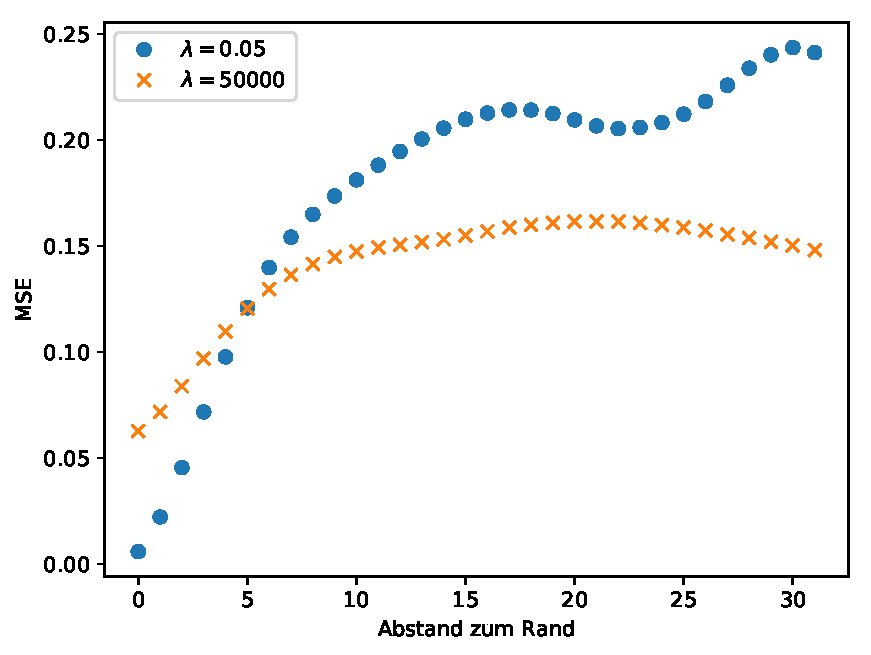
\includegraphics[height=2.5in]{figures/results/inner_cross_prediction/inner_errors.pdf}
	\setcapmargin[1cm]{0.5cm}
	\caption{Graphische Darstellung der Abhängigkeit des MSE für die Vorhersage der $u$-Variable des \textit{Barkley}-Modells vom Abstand zum Rand. In blau ist die Abhängigkeit für das \textsc{ESN}s mit starker und in orange für das mit schwacher Regularisierung dargestellt.}
	\label{fig:exp_inner_cross_barkley_esn_error_dependency_comparison}
\end{figure} 

Um den Einfluss der Regularisierung hervorzuheben sind in Abbildung \ref{fig:exp_inner_cross_barkley_esn_comparison} die Vorhersagen des optimalen Reservoir mit der hohen Regularisierung ($\lambda=\num{5e4}$) und eines zuvor ermittelten Reservoirs mit einer geringeren Regularisierung ($\lambda=0.05$) exemplarisch für das \textit{Barkley}-Modell dargestellt. Es ist zu erkennen, dass im Falle der starken Regularisierung die Vorhersage stark verschwommen ist und beinahe der Mittelwert der Erregung anstelle der feineren Strukturen vorhergesagt wird. Dagegen wird bei der geringeren Regularisierung eine feinere Struktur vorhergesagt. \improvement{Add details?}
Zudem ist in Abbildung \ref{fig:exp_inner_cross_barkley_esn_error_dependency_comparison} die Abhängigkeit des mittleren quadratischen Fehlers für jene beiden Reservoirs dargestellt. Dabei ist zu erkennen, dass im für geringe Abstände die feine Vorhersage mit der kleinen Regularisierung deutlich geringere Fehler verursacht, wohingegen ab einem Abstand von $5$ Gitterpunkten eine stärkere Regularisierung geringere Fehler erzeugt. Zudem scheint der Fehler dabei schnell gegen eine obere Schranke zu konvergieren. Dies lässt sich damit vereinbaren, dass dieses Reservoir hauptsächlich noch den Mittelwert der Dynamik vorhersagt.

\begin{figure}[h]
	\centering
	\begin{subfigure}{.5\textwidth}
		\centering
		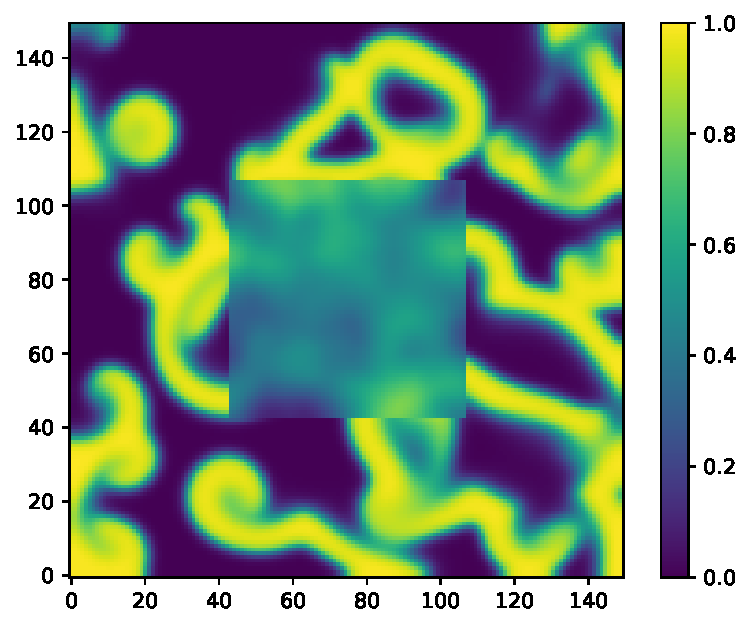
\includegraphics[height=2.5in]{figures/results/inner_cross_prediction/barkley_u_inner_esn_high_penalty.pdf}
		\setcapmargin[1cm]{0.5cm}
		\caption{Vorhersage des \textsc{ESN}s mit $\lambda=50000$}
	\end{subfigure}%
	\begin{subfigure}{.5\textwidth}
		\centering
		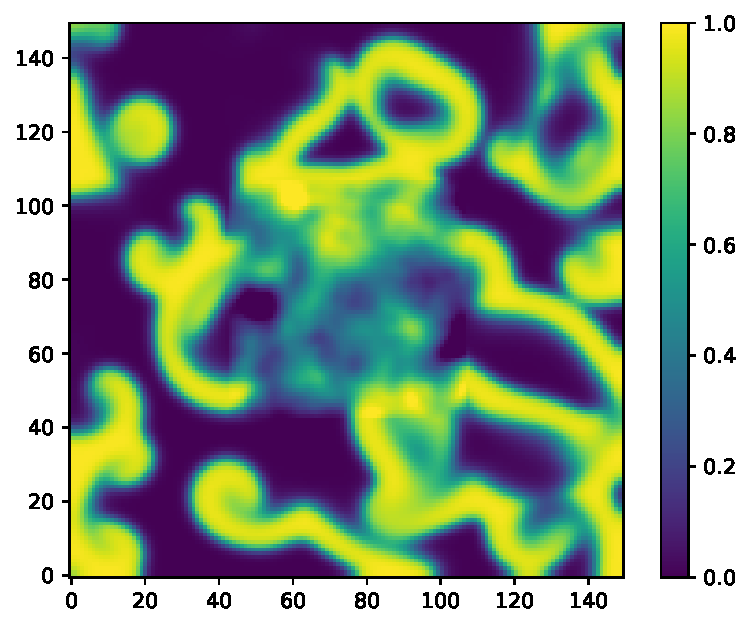
\includegraphics[height=2.5in]{figures/results/inner_cross_prediction/barkley_u_inner_esn_low_penalty.pdf}
		\setcapmargin[1cm]{0.5cm}
  		\caption{Vorhersage des \textsc{ESN}s mit $\lambda=0.05$}
	\end{subfigure}
	\caption{Graphische Darstellung der $u$-Variable des \textit{Barkley}-Modells für den $1000$. Zeitschritt des Evaluationsdatensatzes. Links ist die Vorhersagen des \textsc{ESN}s mit starker und rechts mit schwacher Regularisierung dargestellt.}
	\label{fig:exp_inner_cross_barkley_esn_comparison}
\end{figure} 

\subsection{Vergleich}
Für einen Vergleich der drei Methoden bietet es sich an die Ergebnisse für die größten Wert für $a$ durchzuführen, der mit allen drei Ansätzen betrachtet worden ist. Dies entspricht dem Wert $a=64$. Eine Übersicht der verschiedenen Ergebnisse ist in Tabelle \ref{tab:exp_inner_cross_comparison_results} zu finden.

\begin{table}[h]
	\centering
	\captionsetup{width=0.9\linewidth}
	\begin{tabular}{cccccccc}
		\hline
		\multicolumn{1}{c}{} & \multicolumn{3}{c}{Barkley} & \multicolumn{3}{c}{Mitchell-Schaeffer}		\\
		%\cline{2-7}
		\multicolumn{1}{c}{} & NN & RBF & ESN & NN & RBF & ESN \\
		
		\hline
		
		Laufzeit [s] 	& 20272 	& 1756		& \textbf{1089}		& 14754		&  	1845	& \textbf{1206} \\
		MSE 			& 0.09284	& 0.05588	& 	\textbf{0.05389} 		& 0.24599	& 0.13615 	& \textbf{0.12975}	 \\
		NRMSE 			& 1.1837	& 0.9184	& \textbf{0.9019} 			& 1.3042	& 0.9703 	& \textbf{0.9472} \\
		\hline 
	\end{tabular} 
	\caption{Vergleich der benötigten Laufzeit und der erreichten Fehlers der drei Ansätze für das \textit{Mitchell-Schaeffer}- und das \textit{Barkley}-Modell, welche zu den geringsten Fehlern führen, für $a=64$.}
	\label{tab:exp_inner_cross_comparison_results}
\end{table}

Es zeigt sich erneut, dass die Vorhersagen der klassischen Methoden einen höheren Fehler haben. Während der \textsc{NN}-Ansatz bei beiden Modellen schlechtere Ergebnisse als die Vorhersage mittels des Mittelwertes liefert, sind die radialen Basisfunktionen und die \textsc{ESN}s leicht besser als diese. Dabei erreichen die \textsc{ESN}s und radialen Basisfunktionen in etwa die gleiche Genauigkeit. Diese reicht allerdings auch nicht aus, um dies Methoden tatsächlich sinnvoll verwenden zu können. 

Des Weiteren wächst der Fehlers mit steigender Größe des vorherzusagenden Bereiches auch bei allen drei Ansätze an. Es ist somit zu vermuten, dass dies nicht nur eine reine Beschränkung der einzelnen Methoden ist, sondern dass es womöglich eine Eigenschaft der betrachteten Modelle ist. 
\improvement{Add comparison images}

\begin{figure}[h]
	\centering
	\begin{subfigure}{.5\textwidth}
		\centering
		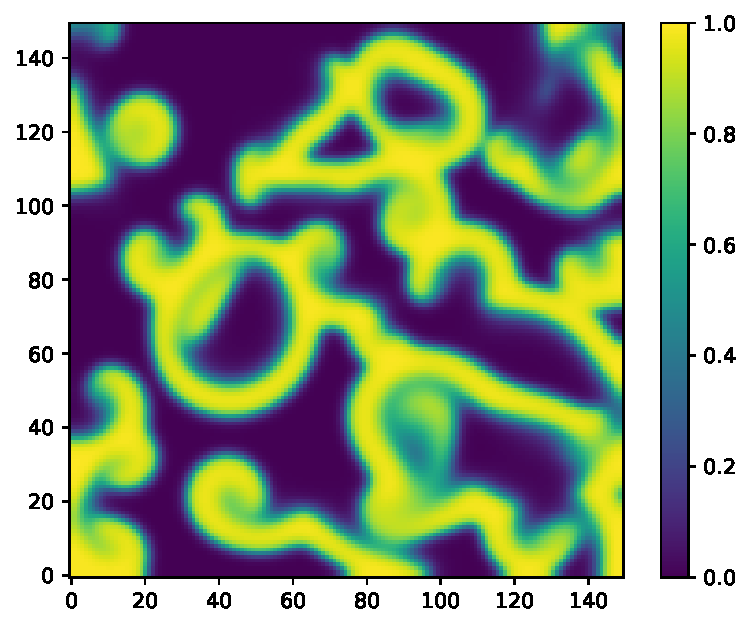
\includegraphics[height=2.5in]{figures/results/inner_cross_prediction/barkley_u_inner_original.pdf}
		\setcapmargin[1cm]{0.5cm}
		\caption{Echte Erregung des Modells}
		\label{fig:exp_inner_cross_barkley_result_orig}
	\end{subfigure}%
	\begin{subfigure}{.5\textwidth}
		\centering
		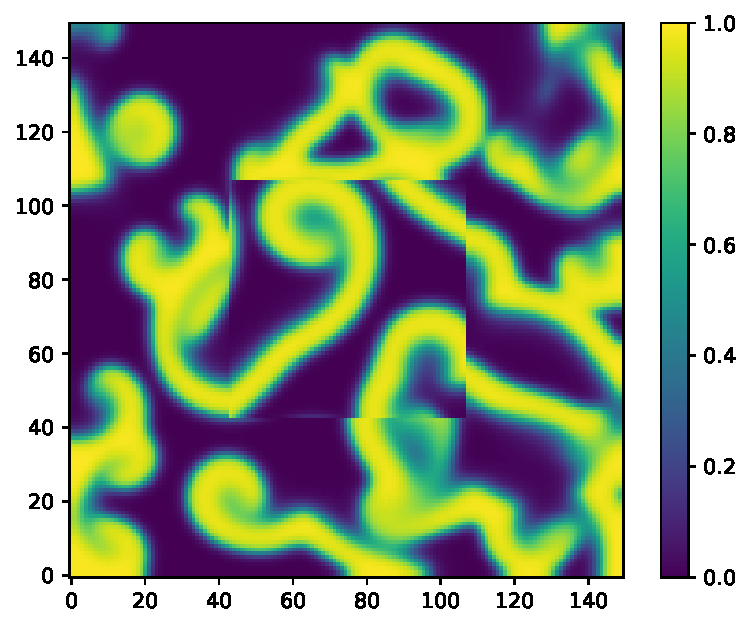
\includegraphics[height=2.5in]{figures/results/inner_cross_prediction/barkley_u_inner_nn.pdf}
		\setcapmargin[1cm]{0.5cm}
  		\caption{Vorhersage des \textsc{NN}-Ansatzes}
  		\label{fig:exp_inner_cross_barkley_result_nn_pred}
	\end{subfigure}
	\begin{subfigure}{.5\textwidth}
		\centering
		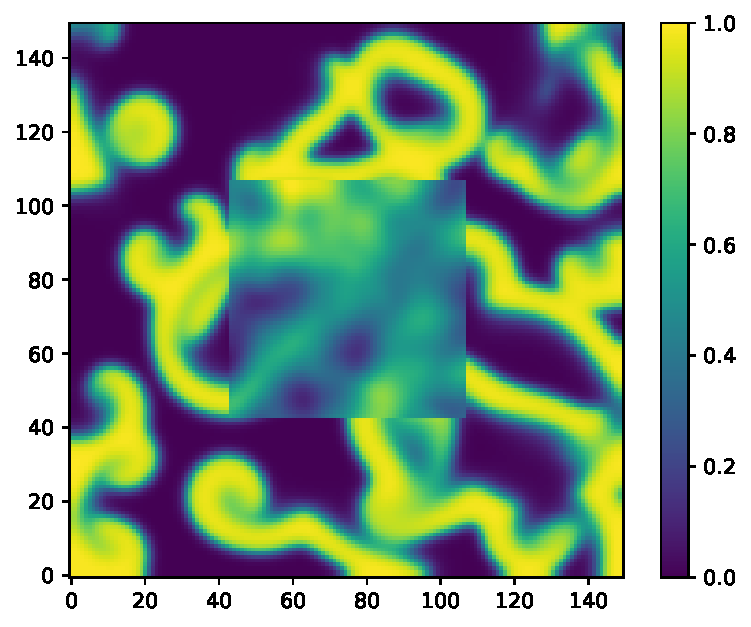
\includegraphics[height=2.5in]{figures/results/inner_cross_prediction/barkley_u_inner_rbf.pdf}
		\setcapmargin[1cm]{0.5cm}
  		\caption{Vorhersage des \textsc{RBF}-Ansatzes}
  		\label{fig:exp_inner_cross_barkley_result_rbf_pred}
	\end{subfigure}%
	\begin{subfigure}{.5\textwidth}
		\centering
		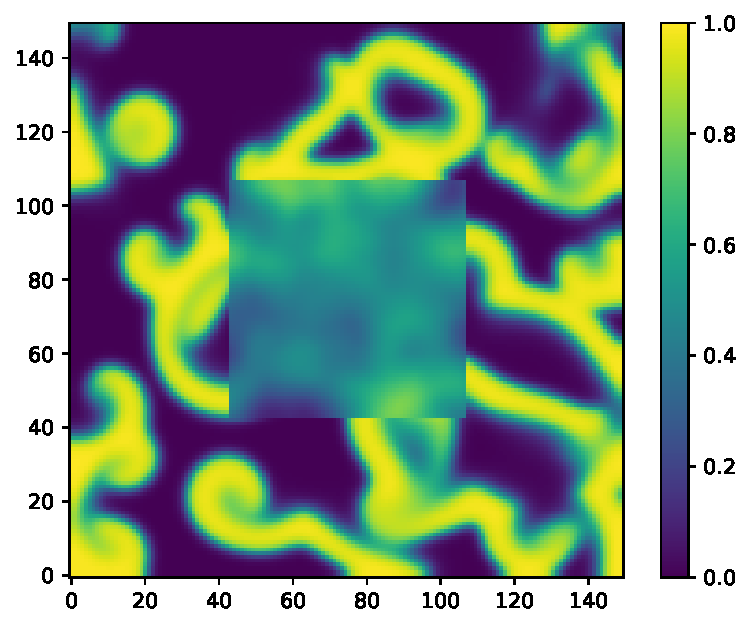
\includegraphics[height=2.5in]{figures/results/inner_cross_prediction/barkley_u_inner_esn.pdf}
		\setcapmargin[1cm]{0.5cm}
  		\caption{Vorhersage des \textsc{ESN}}
  		\label{fig:exp_inner_cross_barkley_result_esn_pred}
	\end{subfigure}
	\caption{Graphische Darstellung der $u$-Variable des \textit{Barkley}-Modells für den $1000$. Zeitschritt des Evaluationsdatensatzes für $a=64$. Oben links ist das tatsächliche Feld des Modells zu sehen. Danach folgenden im Uhrzeigersinn die Vorhersagen des \textsc{NN}-Ansatzes, des \textsc{RBF}-Ansatzes und des \textsc{ESN}.}
	\label{fig:exp_inner_cross_barkley_result}
\end{figure} 

In Abbildung \ref{fig:exp_inner_cross_barkley_result} werden exemplarisch die aus den drei Ansätzen resultierenden Felder der Spannungsvariable $u(t)$ des \textit{Barkley}-Modells zusammen mit dem originalen Feld dargestellt. Eine analoge Darstellung für das \textit{Mitchell-Schaeffer}-Modell ist im Anhang als Abbildung \ref{fig:apx_inner_cross_mitchell_result} zu finden. Es fällt auf, dass sowohl die Vorhersage der \textsc{RBF} als auch die des \textsc{ESN} stark verschwommen sind und kaum Details zeigen. Im Gegensatz dazu gibt der \textsc{NN}-Ansatz eine sehr scharfe Vorhersage. Dies ist dahingehend interessant, als das zum einen jeder Bildpunkt einzeln vorhersagt wird, und zum anderen immer die nächsten fünf Nachbarn genutzt werden. Daraus können zwei Konsequenzen folgen. Erstens spricht die hohe Auflösung dafür, dass die Vorhersage beinahe perfekt ein Bereich aus den Trainingsdaten ist. Da die Vorhersage aber (zumindest in diesem Moment) nicht gut mit dem Original übereinstimmt bedeutet dies, dass die Verzögerungskoordinaten, die genutzt worden sind, den Bereich nicht eindeutig beschreiben. Zweitens kann daraus auch gefolgert werden, dass für diese Aufgabe die Länge der Trainingsdaten zu gering gewählt worden ist. 

\chapter{Diskussion}
\chapter{Fazit}
In dieser Arbeit ist die Anwendung von \textit{Echo State Networks} für die Vorhersage von raumzeitlichen Dynamiken erregbarer Systeme untersucht worden. Dies ist anhand des \textit{Barkley}- und des \textit{Mitchell-Schaeffer}-Modells durchgeführt worden. Für die Vorhersage dieser raumzeitlichen Dynamiken ist ein sogenannter \textit{Messsonendenansatz} entwickelt und verwendet worden, bei dem nur lokal benachbarte Informationen für die Vorhersage genutzt werden.\\

Um die experimentellen Ergebnisse des \textsc{ESN}s einzuordnen, sind sie mit den Ergebnissen eines \textit{nächsten Nachbar}-Ansatzes und \textit{radialer Basisfunktionen} verglichen worden. Dabei sind Anwendungsarten betrachtet worden, welche für die Untersuchung von Herzen relevant sind: Zuerst ist eine nicht gemessene aus einer gemessenen Systemvariable bestimmt worden. Anschließend ist die elektrische Erregung auf der Herzoberfläche anhand des Fernfelds einer Elektrodenmessung rekonstruiert worden. Abschließend ist versucht worden die elektrische Erregung für unbekannte Regionen aus der Kenntnis weniger Randwerte vorzunehmen.\\

Es halt sich allgemein gezeigt, dass durch die Verwendung der \textit{Echo State Networks} in jedem Anwendungsbereich eine größere Genauigkeit erzielt werden konnte. Die \textsc{ESN}s stellen eine gut geeignete Methode zur Untersuchung und Vorhersage raumzeitlicher Dynamiken erregbarer Medien dar. Diese Erkenntnis passt zu den neusten wissenschaftlichen Publikationen auf dem Bereich \citep{Lu2017}.\\

Im Detail konnte die Kreuz-Prädiktion zwischen den zwei Systemvariablen nahezu fehlerfrei gelöst werden. Die Rekonstruktion der elektrischen Erregung konnte zudem die makroskopische Struktur der Dynamik rekonstruiert werden, aber nicht die Detailstruktur. Die Vorhersage des unbekannten Bereiches durch die Randwerte konnte nicht zufriedenstellend gelöst werden. Bereits für geringe Größen des vorherzusagenden Bereichs stieg der Fehler sowohl bei dem \textsc{ESN} als auch bei den Referenzmethoden sehr stark an. Dies kann ein Hinweis auf eine generelle physikalische Beschränktheit solcher Voraussagen sein. Es empfiehlt sich dieses Phänomen weitergehend zu untersuchen. \\

Es hat sich zudem herausgestellt, dass die Gewichtsmatrix $\mathbf{W_{out}}$ für verschiedene Bildpunkte eine große Ähnlichkeit aufzeigt. Somit bietet es sich an dieses Verhalten weiter zu untersuchen. Durch die Verwendung einer einzigen Auslesematrix lässt sich die Geschwindigkeit des \textsc{ESN} stark erhöhen. Zusätzlich wäre auch ein Einsatz anderer Methode aus dem Bereich des \textit{Machine Learnings} als Ersatz für die Auslesematrix, wie beispielsweise \textsc{FFNN}s denkbar.  
\section{Ausblick}
Für das Schreiben dieses Berichts hat sich die Wahl der \textsc{LaTeX}-Umgebung als gut geeignet herausgestellt. Die optische Darstellung von mathematischen Ausdrücken sowie des erklärenden Textes ist hierbei intuitiver umzusetzen als bei den bekannten Alternativen. Hierbei wurde die verwendete Literatur über \textsc{Zotero} und \textsc{BibTeX} direkt in den \textsc{LaTeX}-Quellcode eingebunden und zitiert.\\
Für die Literaturrecherche ist der Dienst \textsc{Google Scholar} benutzt worden, welcher eine umfassende Datenbank besitzt.\\

Das Programmieren der Anwendungsbeispiele wurde mit der Sprache \textsc{Python} und den bekannten Frameworks \textsc{Numpy} und \textsc{Scipy} umgesetzt. Diese Entscheidung wurde hauptsächlich durch die große Flexibilität dieser Sprache und der ausreichenden Leistung der Bibliotheken beeinflusst. Die hierbei entstandenen Grafiken wurden mit der \textsc{Pyplot} Bibliothek umgesetzt.\\ 

Dieses gesamte Vorgehen hat sich im Laufe des Praktikums als gut erwiesen und wird somit auch in der anschließenden Bachelorarbeit weiterverfolgt werden.
\chapter{Danksagungen}
Zuerst möchte ich Herrn Professor Ulrich Parlitz für die ausführliche Betreuung und Unterstützung beim Schreiben dieser Bachelorarbeit danken. Zudem möchte ich Herrn Professor Florentin Wörgötter für seine Funktion als Zweitgutachter danken. Des Weiteren möchte ich Thomas Lilienkamp für seine Ratschläge bei technischen Problemen und die hilfreichen Ideenaustausche danken. Zudem bedanke ich mich bei XXX, YYY und ZZZ für das Korrekturlesen dieser Arbeit. 

%\nocite{*}

%\appendix

\cleardoublepage
%% Bibliographie. Das Argument muss der Name der BIBTeX-Datenbank stehen.
%% Ein Beispiel fuer eine solche Datenbank finden Sie in bthesis_datenbank.bib
\bibliography{thesis_datenbank} 

%\chapter*{Danksagung}

%% Dieser Befehl MUSS am Ende stehen und erzeugt die Erklaerung ueber die
%% benutzten Mittel
%\Declaration

\end{document}
